
\section{Análise de Centralidade em Grafos de Conectividade}
\label{sec:analise_centralidade}

Nesta seção, investigamos as principais métricas de centralidade – \emph{betweenness}, \emph{degree} e \emph{eigenvector} – em redes de conectividade construídas a partir das métricas CF-PLM (EEG-ECG) e PLI (EEG-EEG). Cada métrica oferece uma perspectiva distinta sobre a importância dos nós (canais) na rede. Segundo \cite{rubinov2010complex}, regiões cerebrais importantes, denominadas \emph{hubs}, interagem com diversas outras áreas, facilitando a integração funcional e contribuindo para a resiliência da rede frente a danos ou patologias. De forma complementar, \cite{bullmore2009complex} enfatizam que hubs são nós com alta centralidade, essenciais para uma comunicação eficiente entre regiões cerebrais. Esses conceitos fundamentam a escolha e a interpretação das métricas aqui discutidas. As redes foram analisadas nos cenários \emph{com outliers} e \emph{sem outliers}, permitindo avaliar a robustez das estruturas obtidas.

A seguir, descrevemos e interpretamos detalhadamente a métrica de \emph{betweenness centrality} para os dois grupos de rede.

\subsection{Betweenness Centrality}

A \emph{betweenness centrality} mede quantas vezes um nó atua como “ponte” nos caminhos mais curtos entre quaisquer dois nós da rede. Conforme \cite{freeman1977set}, um nó é considerado central quando participa frequentemente dos caminhos mais curtos, facilitando ou controlando a comunicação entre outros nós. Essa métrica é aplicada para identificar canais que funcionam como vias críticas na propagação da informação em redes EEG-ECG e EEG-EEG.

\subsubsection{CF-PLM (EEG-ECG)}
\begin{figure}[htb]
    \centering
    \subfloat[Com Outliers]{
        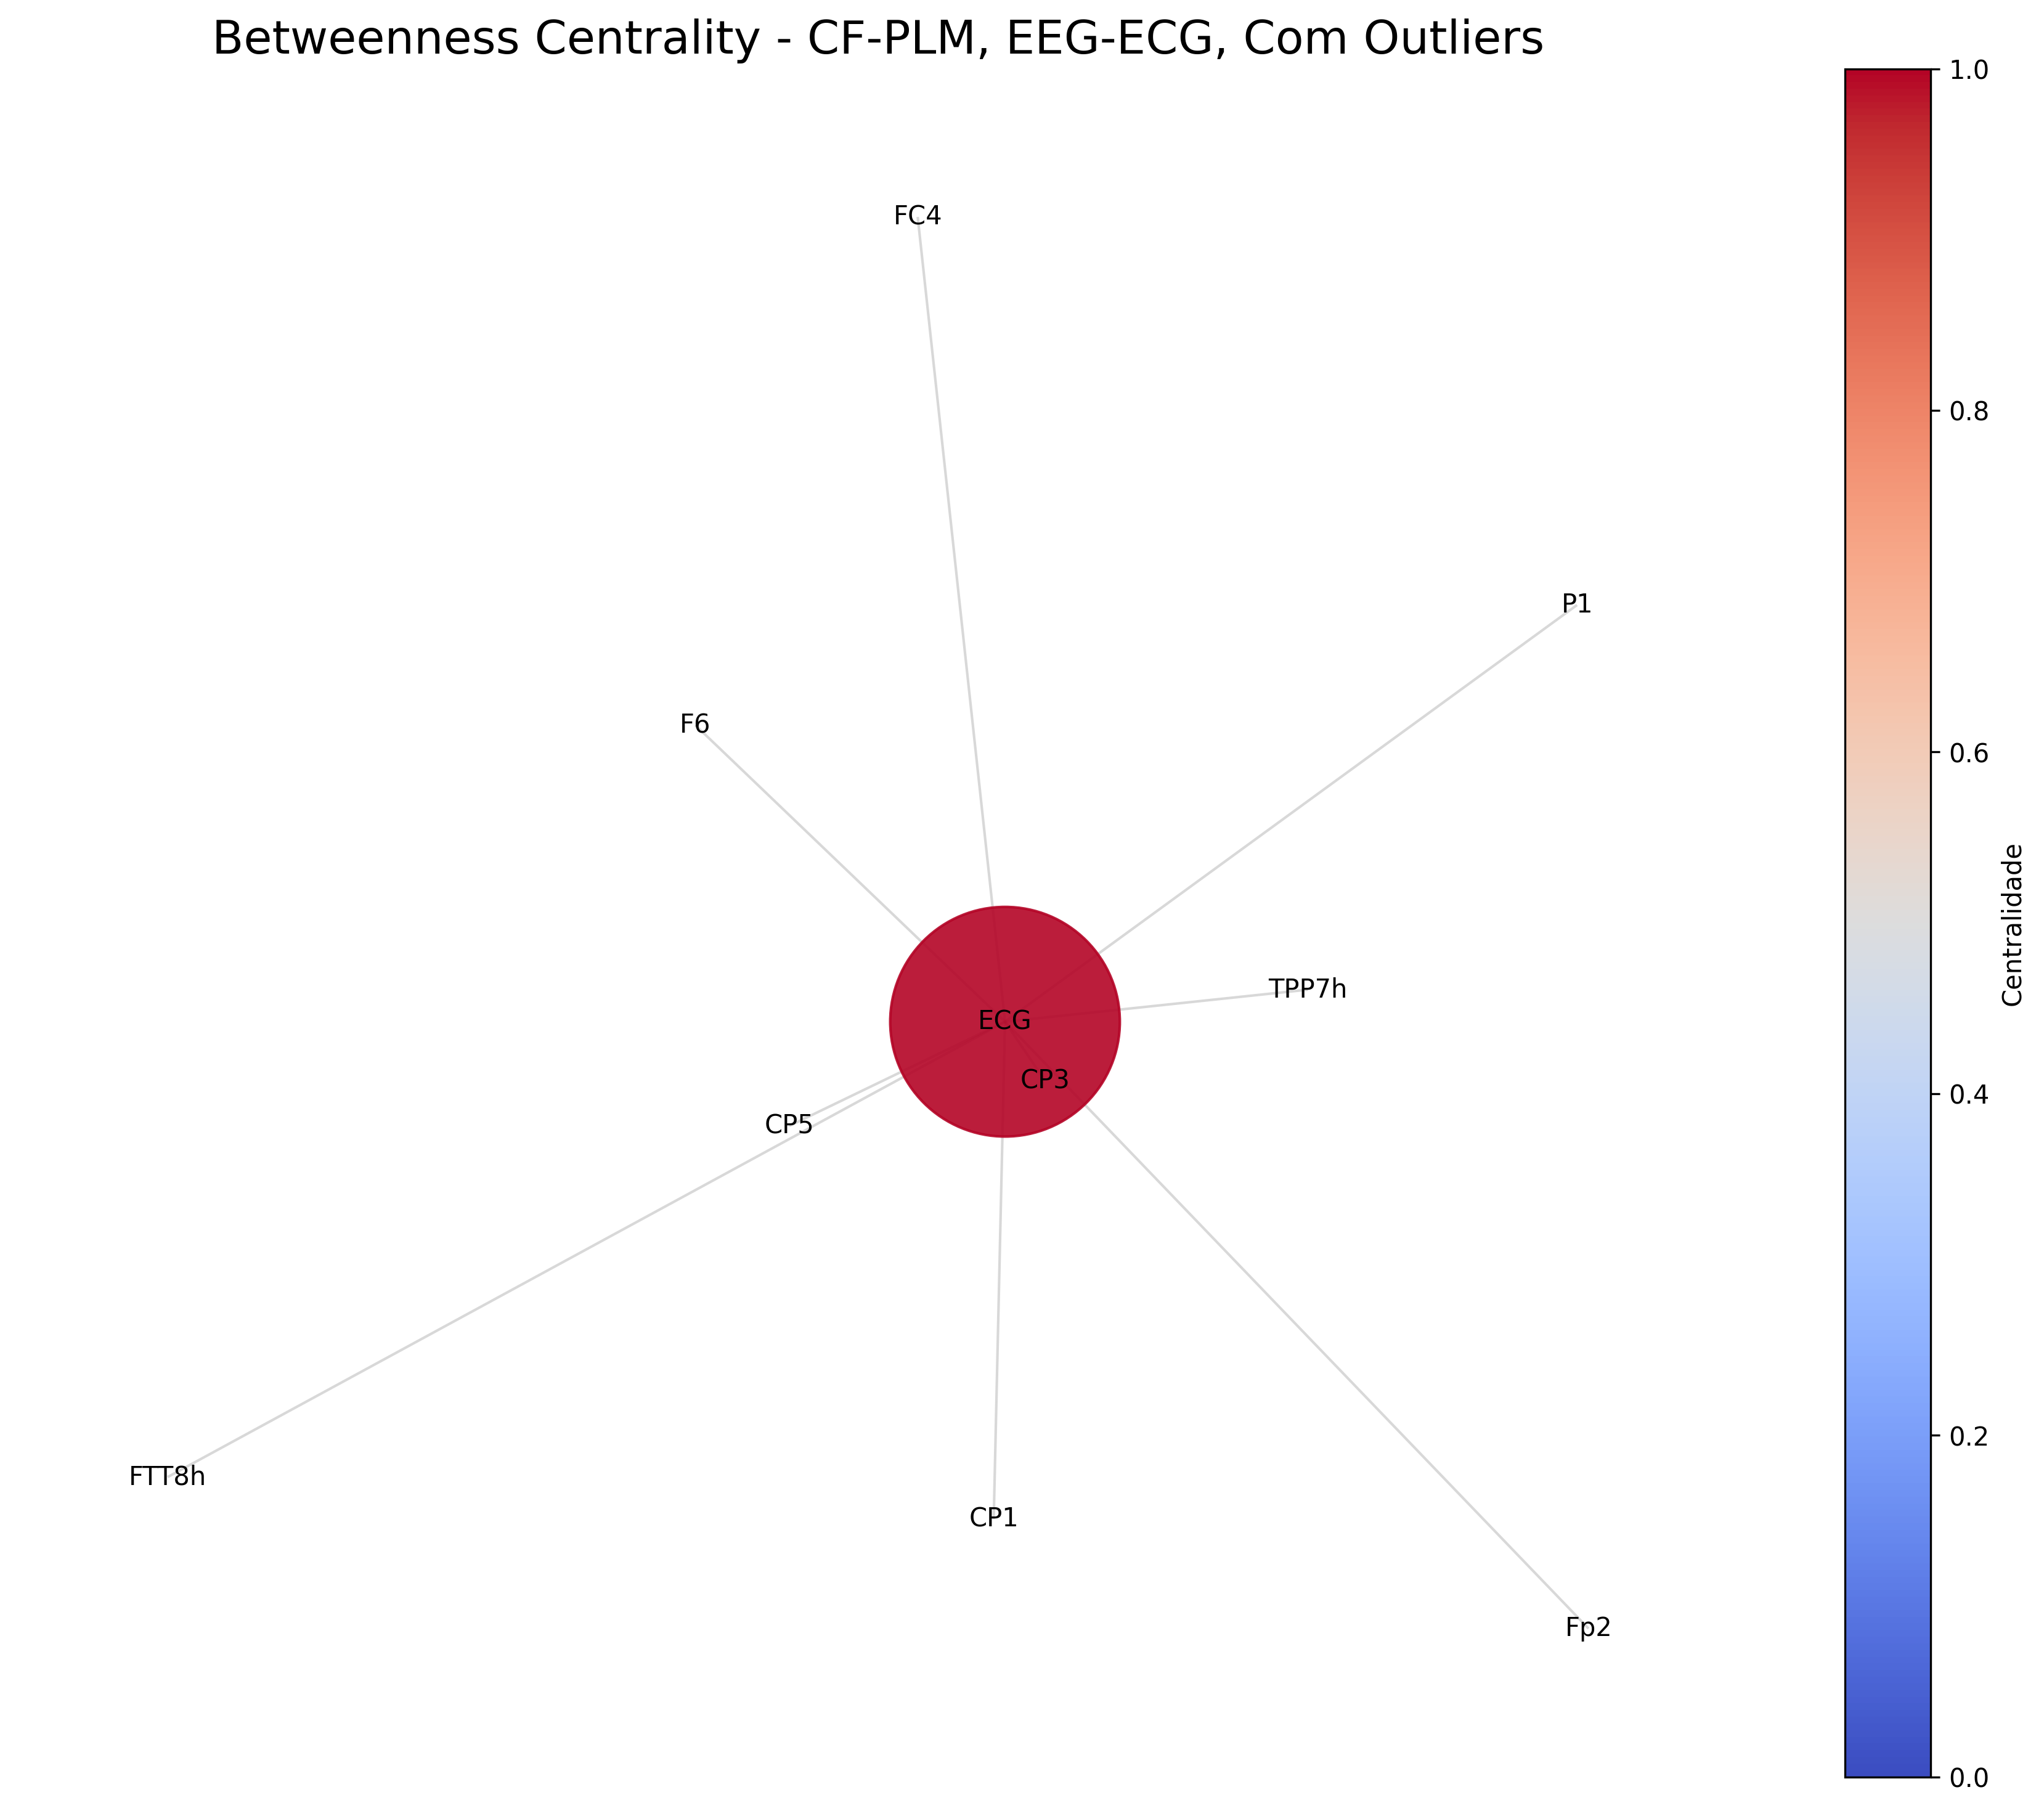
\includegraphics[width=0.45\textwidth]{figs/7_bootstrap_results_analysis/3_centrality_graphs/Betweenness_Centrality__CFPLM_EEGECG_Com_Outliers.png}
        \label{fig:bc_cfplm_eegecg_com}
    }
    \quad
    \subfloat[Sem Outliers]{
        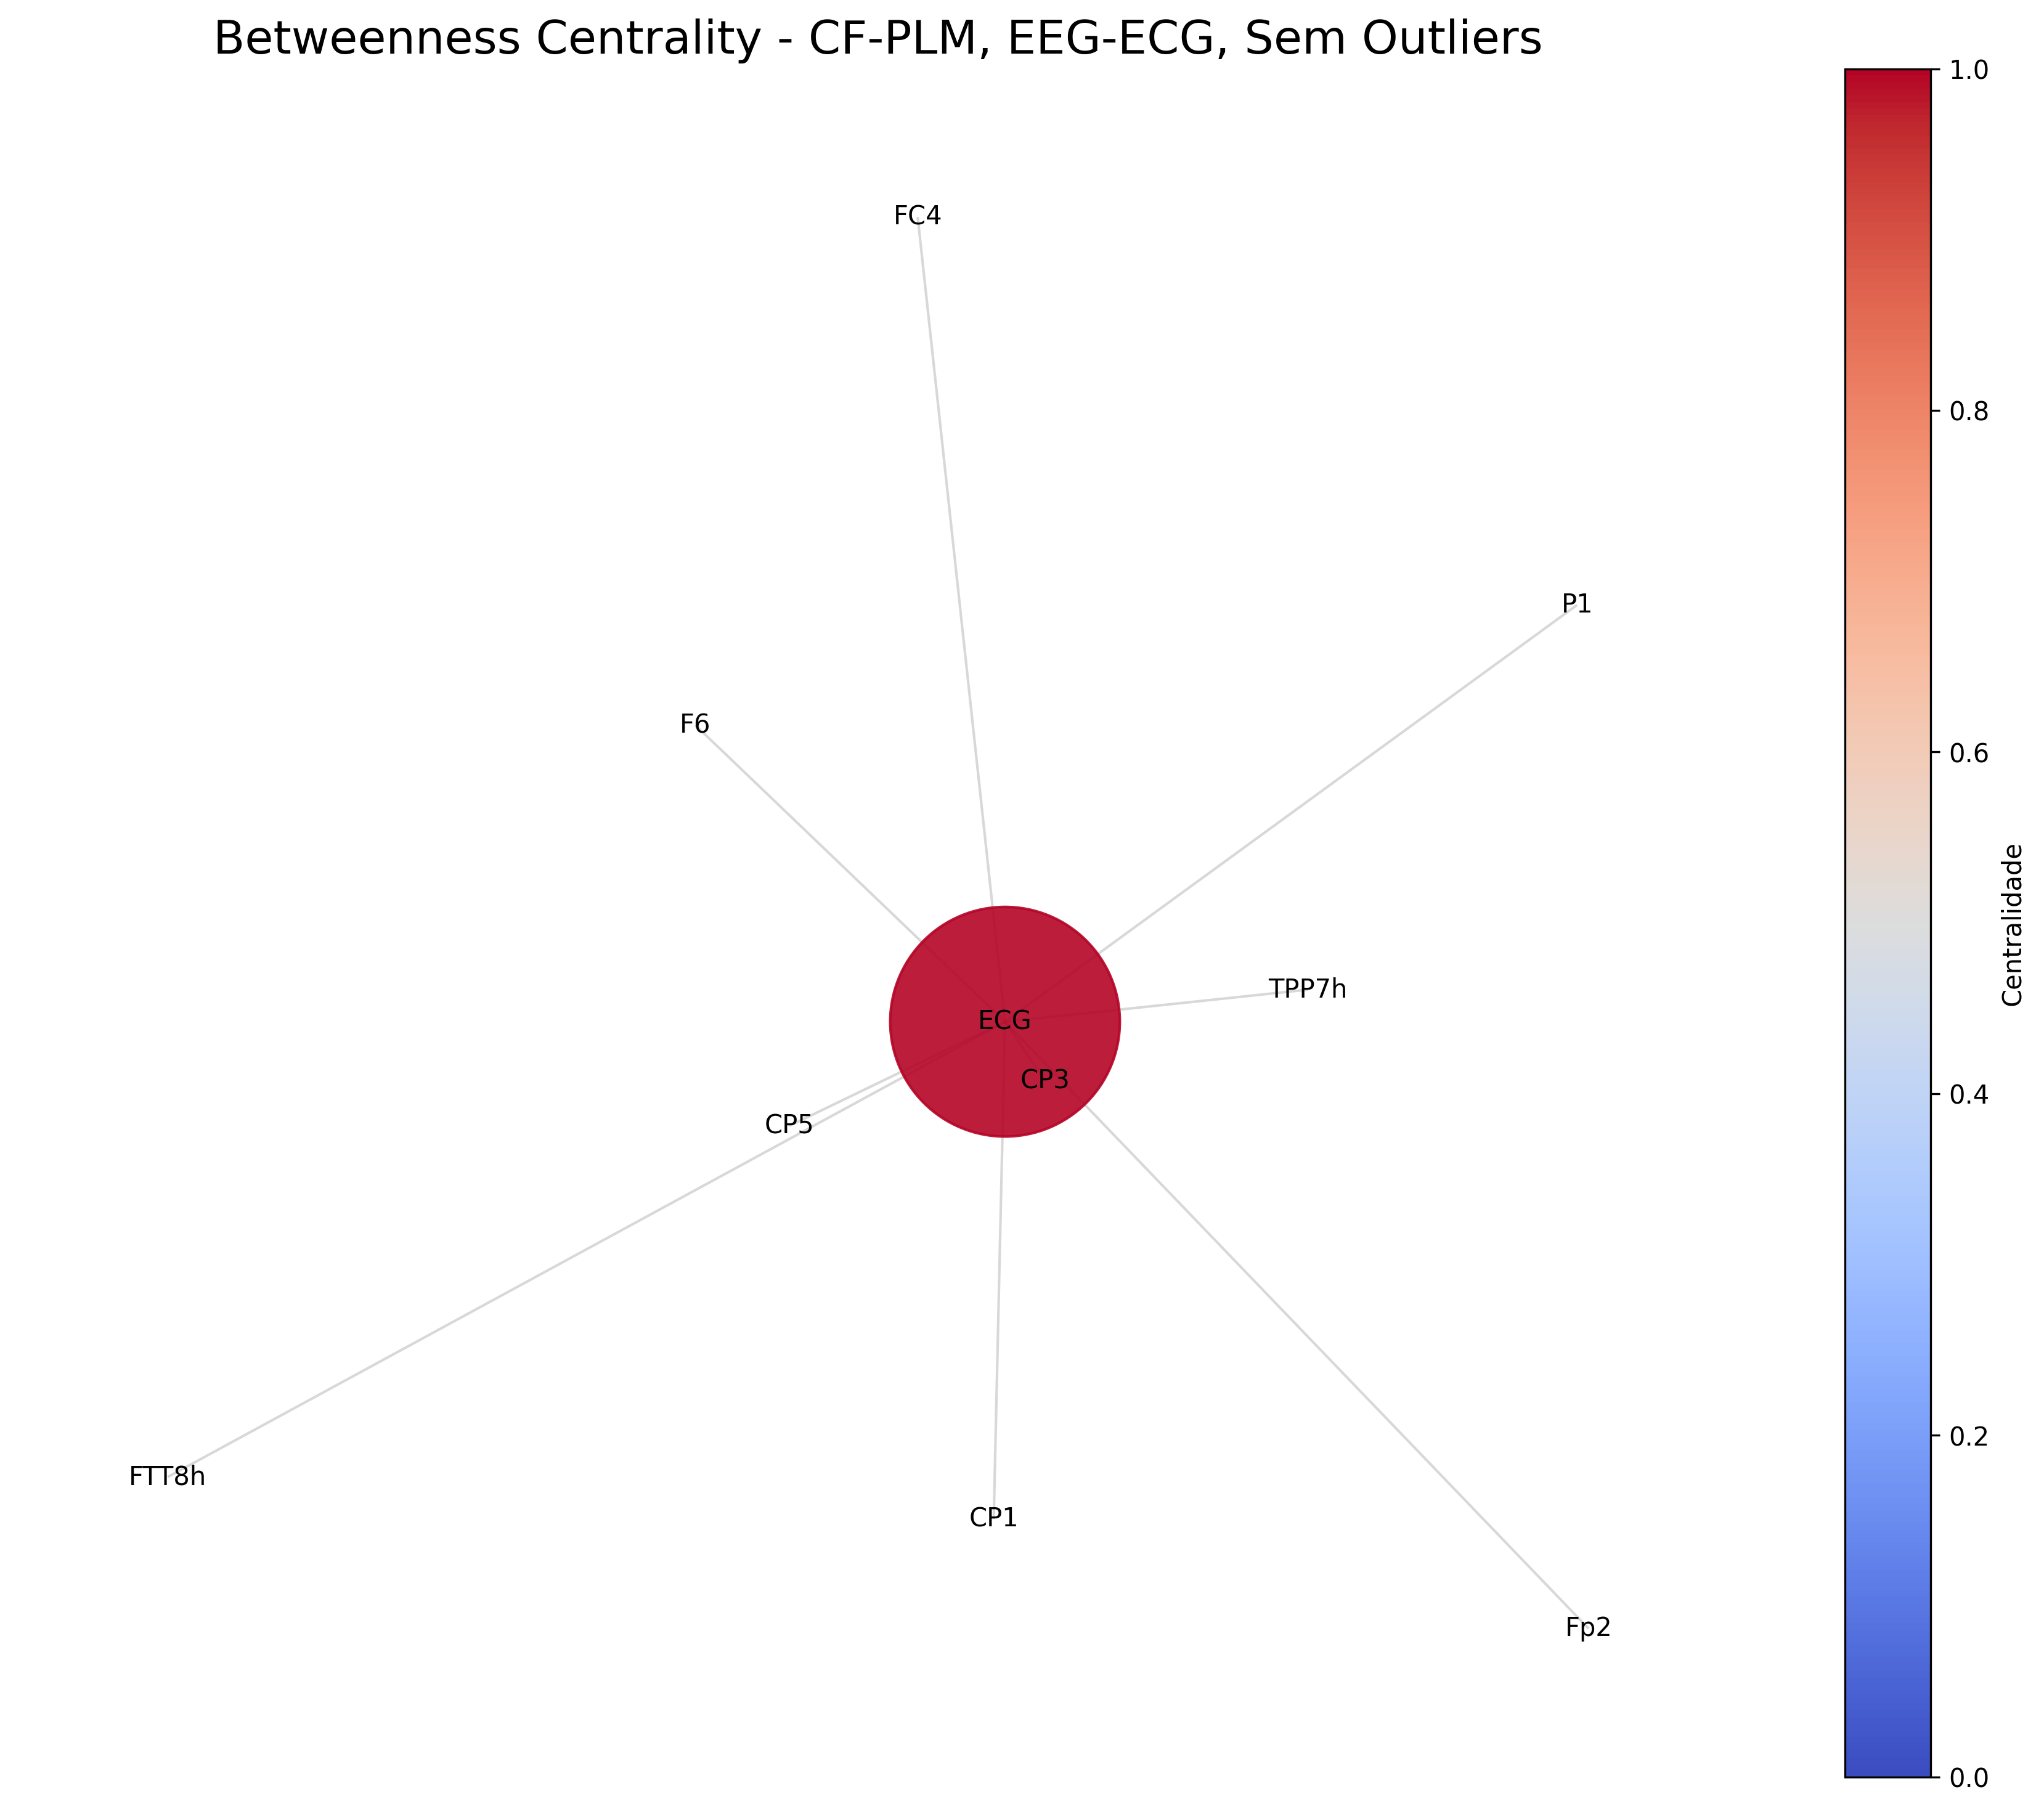
\includegraphics[width=0.45\textwidth]{figs/7_bootstrap_results_analysis/3_centrality_graphs/Betweenness_Centrality__CFPLM_EEGECG_Sem_Outliers.png}
        \label{fig:bc_cfplm_eegecg_sem}
    }
    \caption{Betweenness Centrality no cenário CF-PLM (EEG-ECG). O canal \emph{ECG} domina a rede em ambos os cenários.}
    \label{fig:bc_cfplm_eegecg}
\end{figure}

Nos gráficos da Figura~\ref{fig:bc_cfplm_eegecg}, o canal \emph{ECG} aparece como o nó com maior \emph{betweenness centrality}, pois todas as conexões \emph{cross-frequency} entre EEG e ECG passam por ele. A remoção de outliers não altera substancialmente essa estrutura, mantendo o \emph{ECG} central e evidenciando uma rede “estrela” em torno do canal cardíaco, conforme esperado para acoplamentos cross-frequency \cite{bullmore2009complex}.

\subsubsection{PLI (EEG-EEG)}
\begin{figure}[htb]
    \centering
    \subfloat[Com Outliers]{
        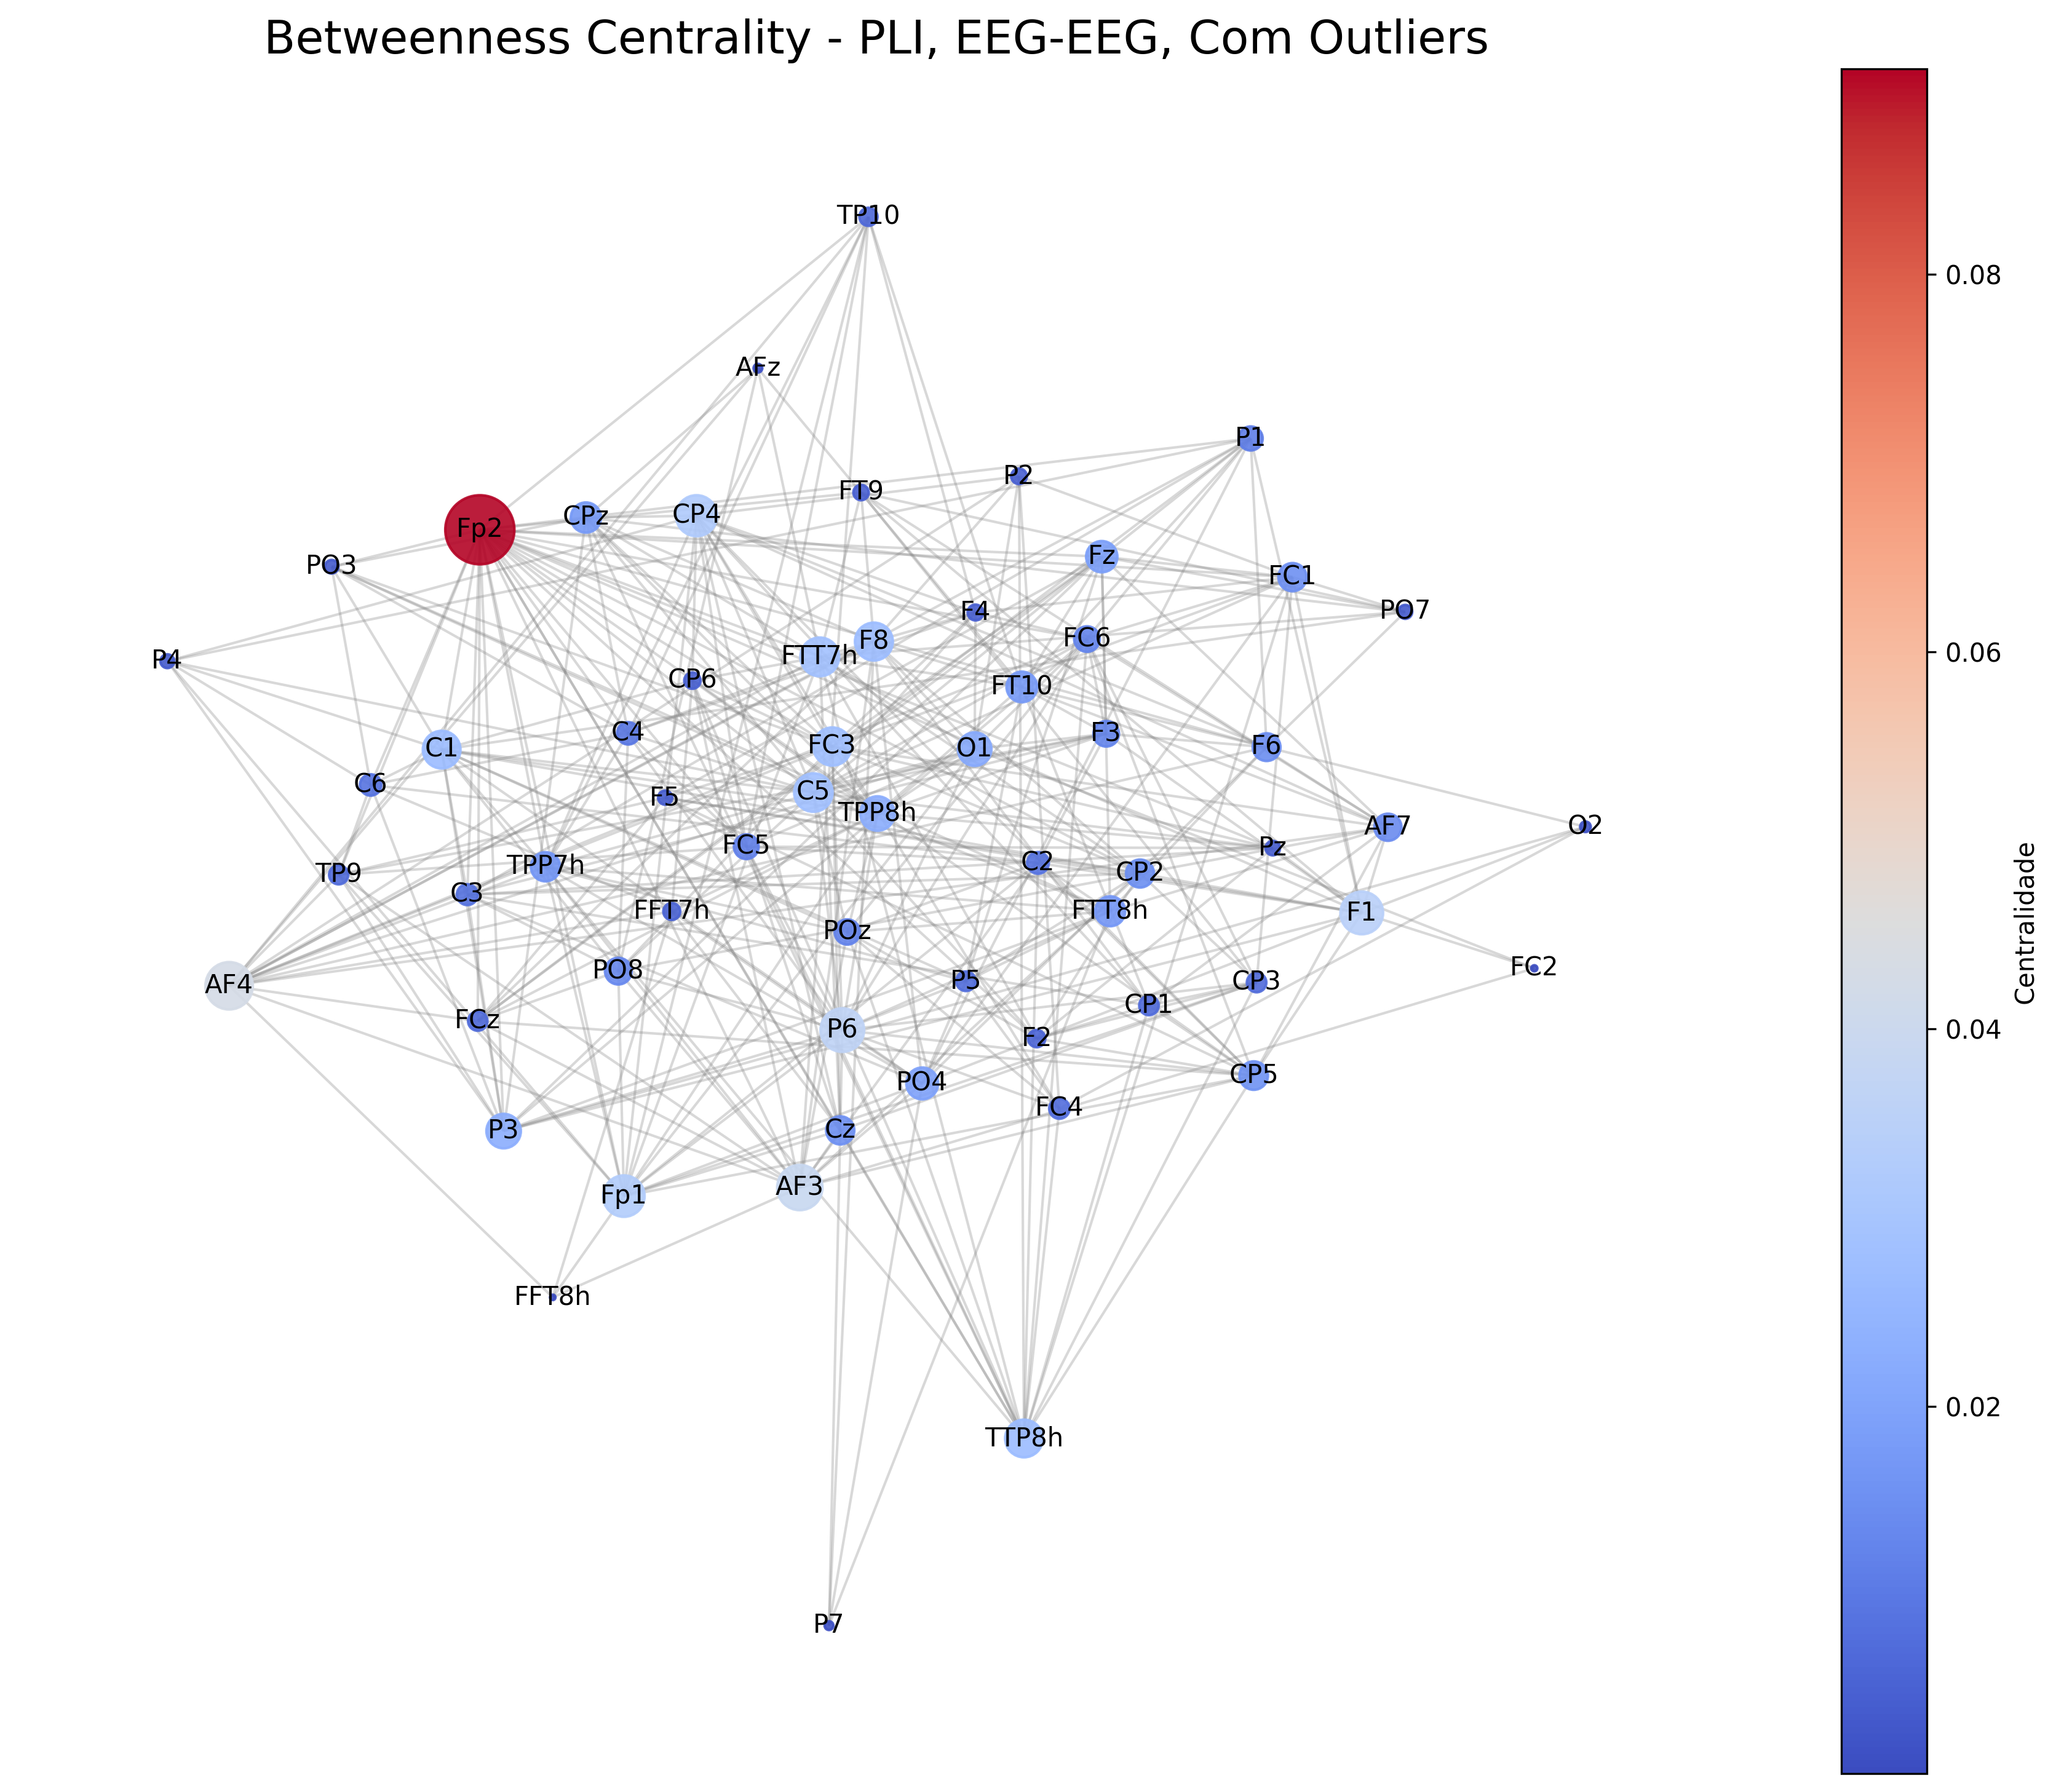
\includegraphics[width=0.45\textwidth]{figs/7_bootstrap_results_analysis/3_centrality_graphs/Betweenness_Centrality__PLI_EEGEEG_Com_Outliers.png}
        \label{fig:bc_pli_eegeeg_com}
    }
    \quad
    \subfloat[Sem Outliers]{
        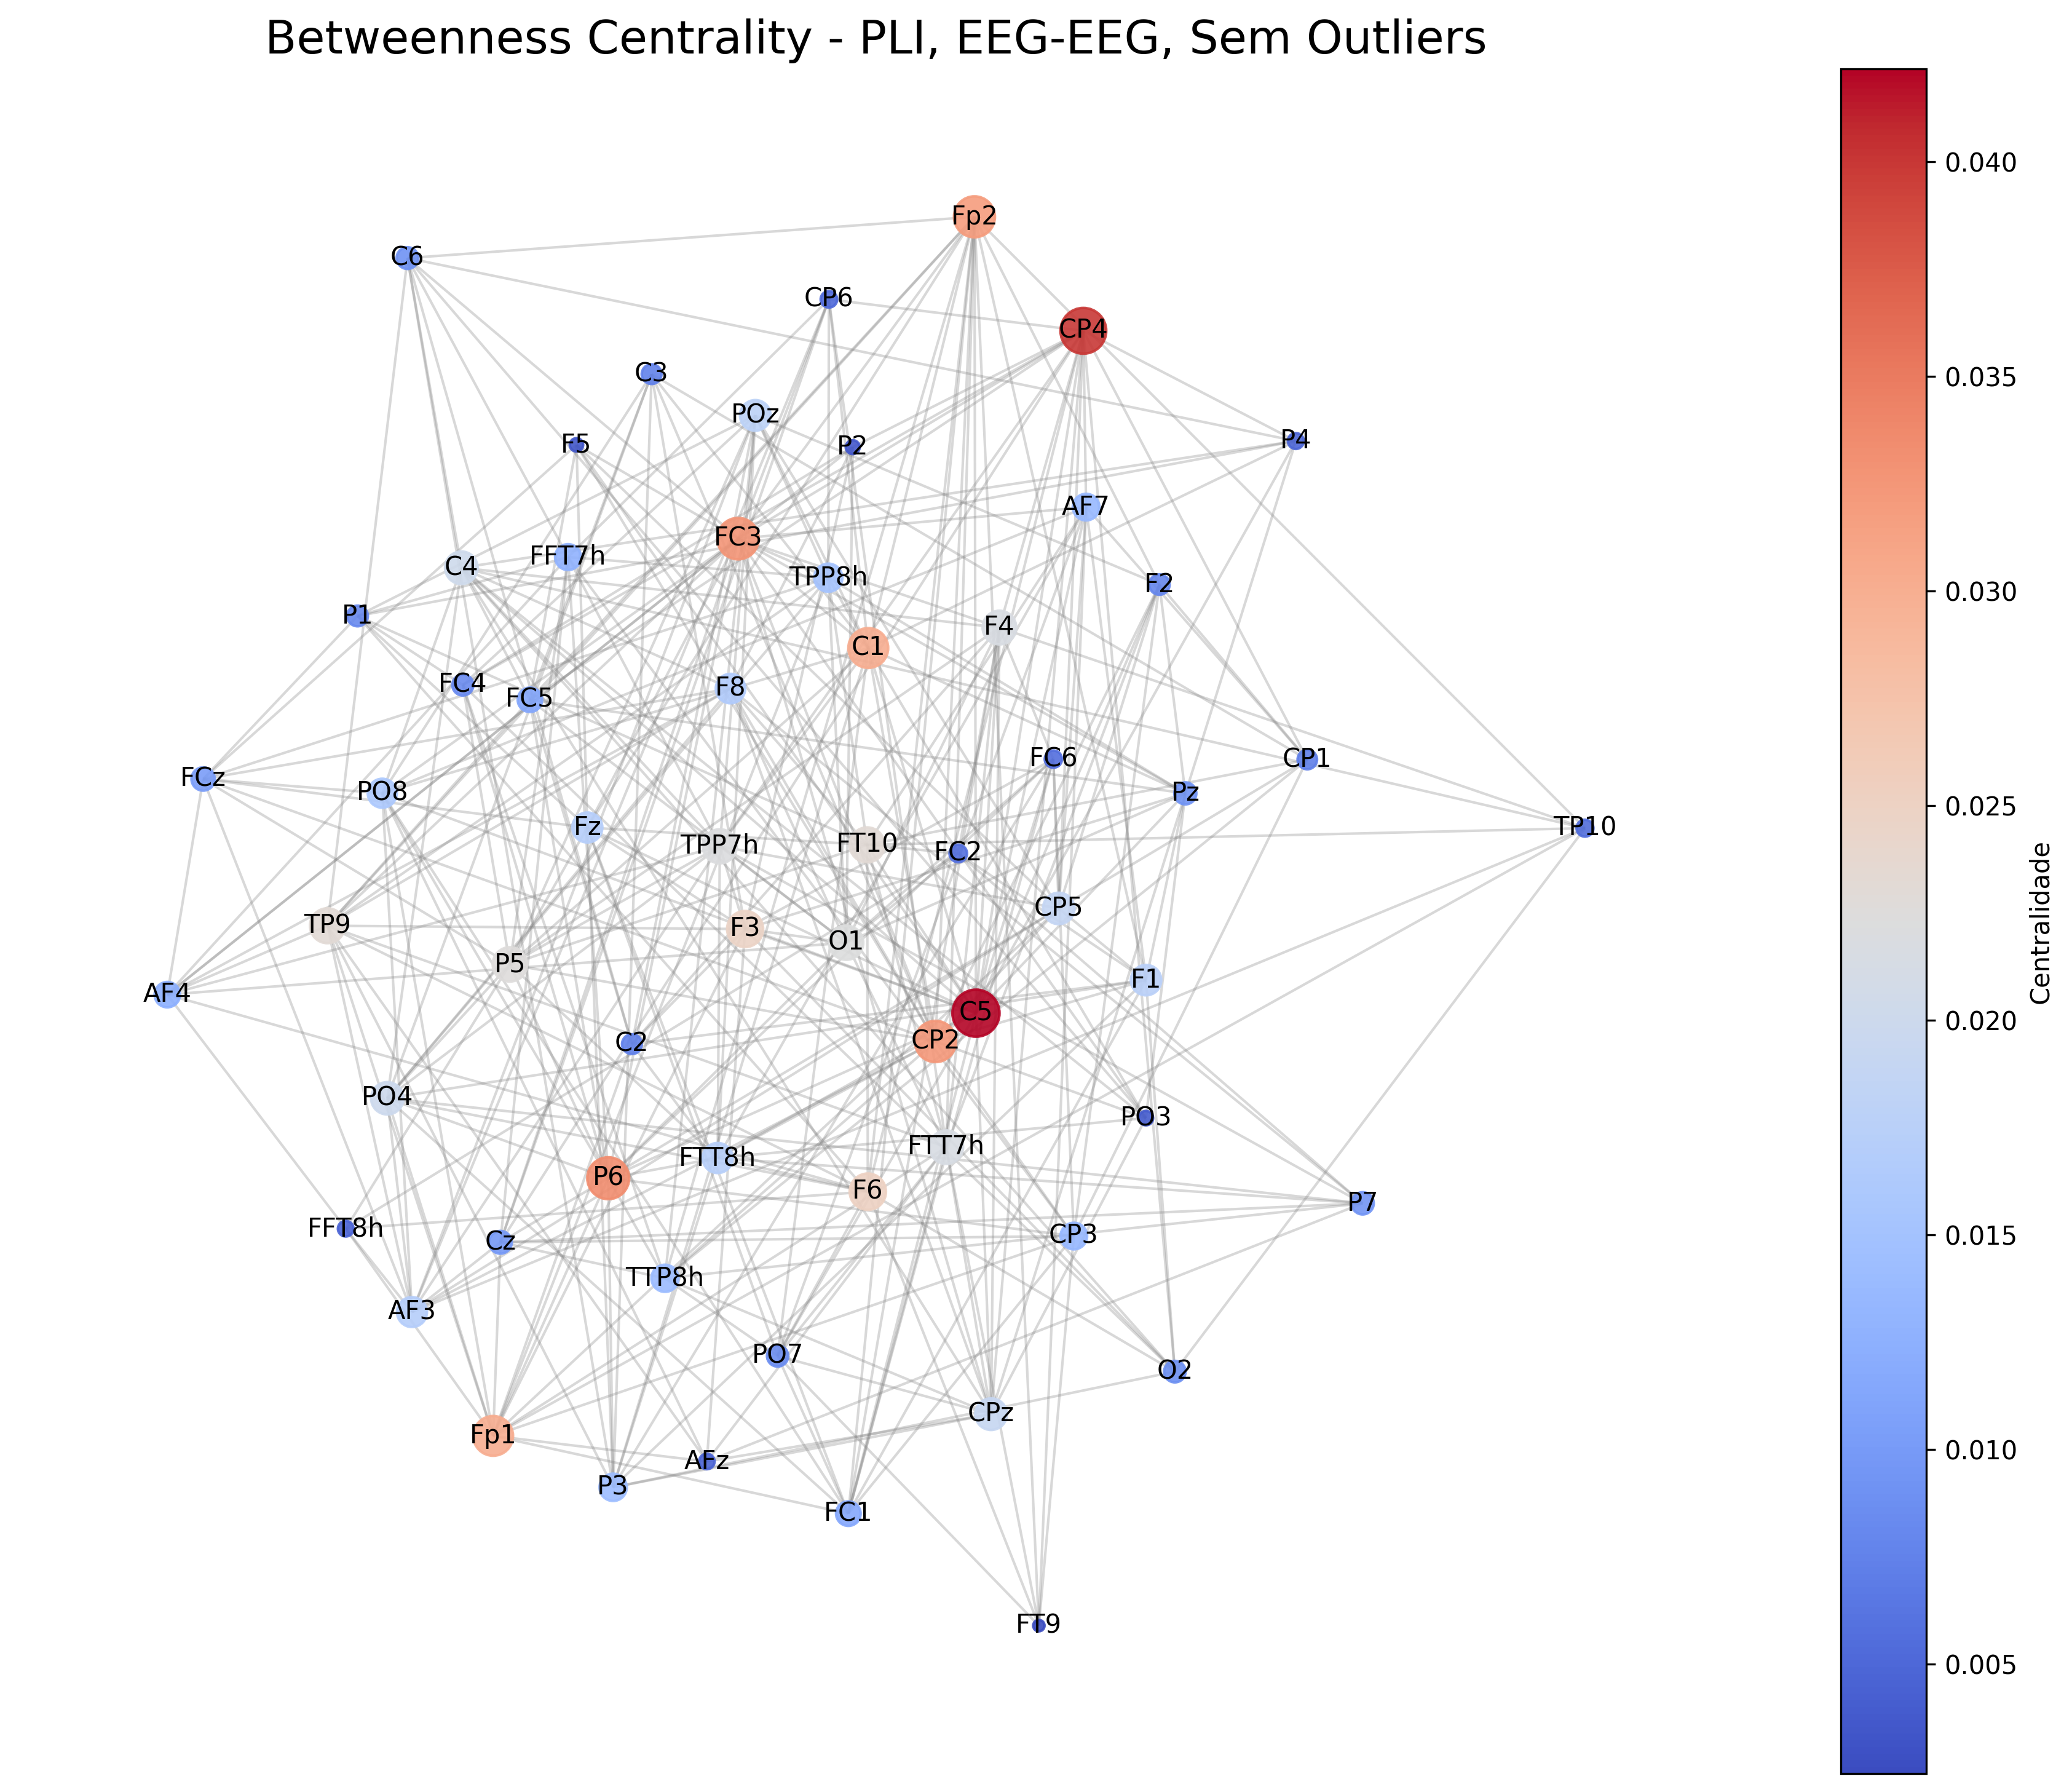
\includegraphics[width=0.45\textwidth]{figs/7_bootstrap_results_analysis/3_centrality_graphs/Betweenness_Centrality__PLI_EEGEEG_Sem_Outliers.png}
        \label{fig:bc_pli_eegeeg_sem}
    }
    \caption{Betweenness Centrality no cenário PLI (EEG-EEG). Canais frontais ou parietais, como Fp2 e CP2, podem se destacar como “pontes” de sincronização.}
    \label{fig:bc_pli_eegeeg}
\end{figure}

Na Figura~\ref{fig:bc_pli_eegeeg}, a rede EEG-EEG apresenta uma estrutura mais complexa, na qual certos canais, como Fp2 e CP2, demonstram alta \emph{betweenness centrality}, atuando como “pontes” para múltiplas conexões. A remoção de outliers não altera drasticamente a centralidade desses canais, sugerindo que as conexões essenciais permanecem estáveis. Esses canais frontais ou parietais podem refletir regiões-chave na sincronização de fase iso-frequencial \cite{rubinov2010complex}.

\subsection{Degree Centrality e Eigenvector Centrality}

(Obs.: A descrição das métricas \emph{degree} e \emph{eigenvector} e suas análises podem ser apresentadas em subseções subsequentes ou no Apêndice, conforme a organização desejada. Neste exemplo, focamos na métrica de betweenness conforme apresentado.)

\subsection{Resumo das Comparações das Métricas de Centralidade}

\begin{itemize}
    \item \textbf{Betweenness Centrality (CF-PLM):} A análise das redes de EEG-ECG mostra que o canal \emph{ECG} é consistentemente o nó central, independentemente da remoção de outliers, refletindo uma rede com topologia de "estrela".
    \item \textbf{Betweenness Centrality (PLI):} Nas redes EEG-EEG, canais como Fp2 e CP2 se destacam como hubs críticos, com a remoção de outliers não alterando substancialmente esses achados.
\end{itemize}

Esses resultados fundamentam as análises topográficas e de rede que serão detalhadas nas seções seguintes.

\subsection{Degree Centrality}

A \emph{degree centrality} contabiliza o número de conexões diretas de cada nó, refletindo sua “popularidade” ou influência imediata na rede. Segundo \cite{newman2010networks}, essa métrica é uma das formas mais simples e diretas para determinar a importância de um vértice, considerando apenas o número de conexões diretas que ele possui. No contexto das redes analisadas (EEG-ECG e EEG-EEG), canais com alto grau são candidatos a serem hubs de informação direta.

\subsubsection{CF-PLM (EEG-ECG)}
\begin{figure}[htb]
    \centering
    \subfloat[Com Outliers]{
        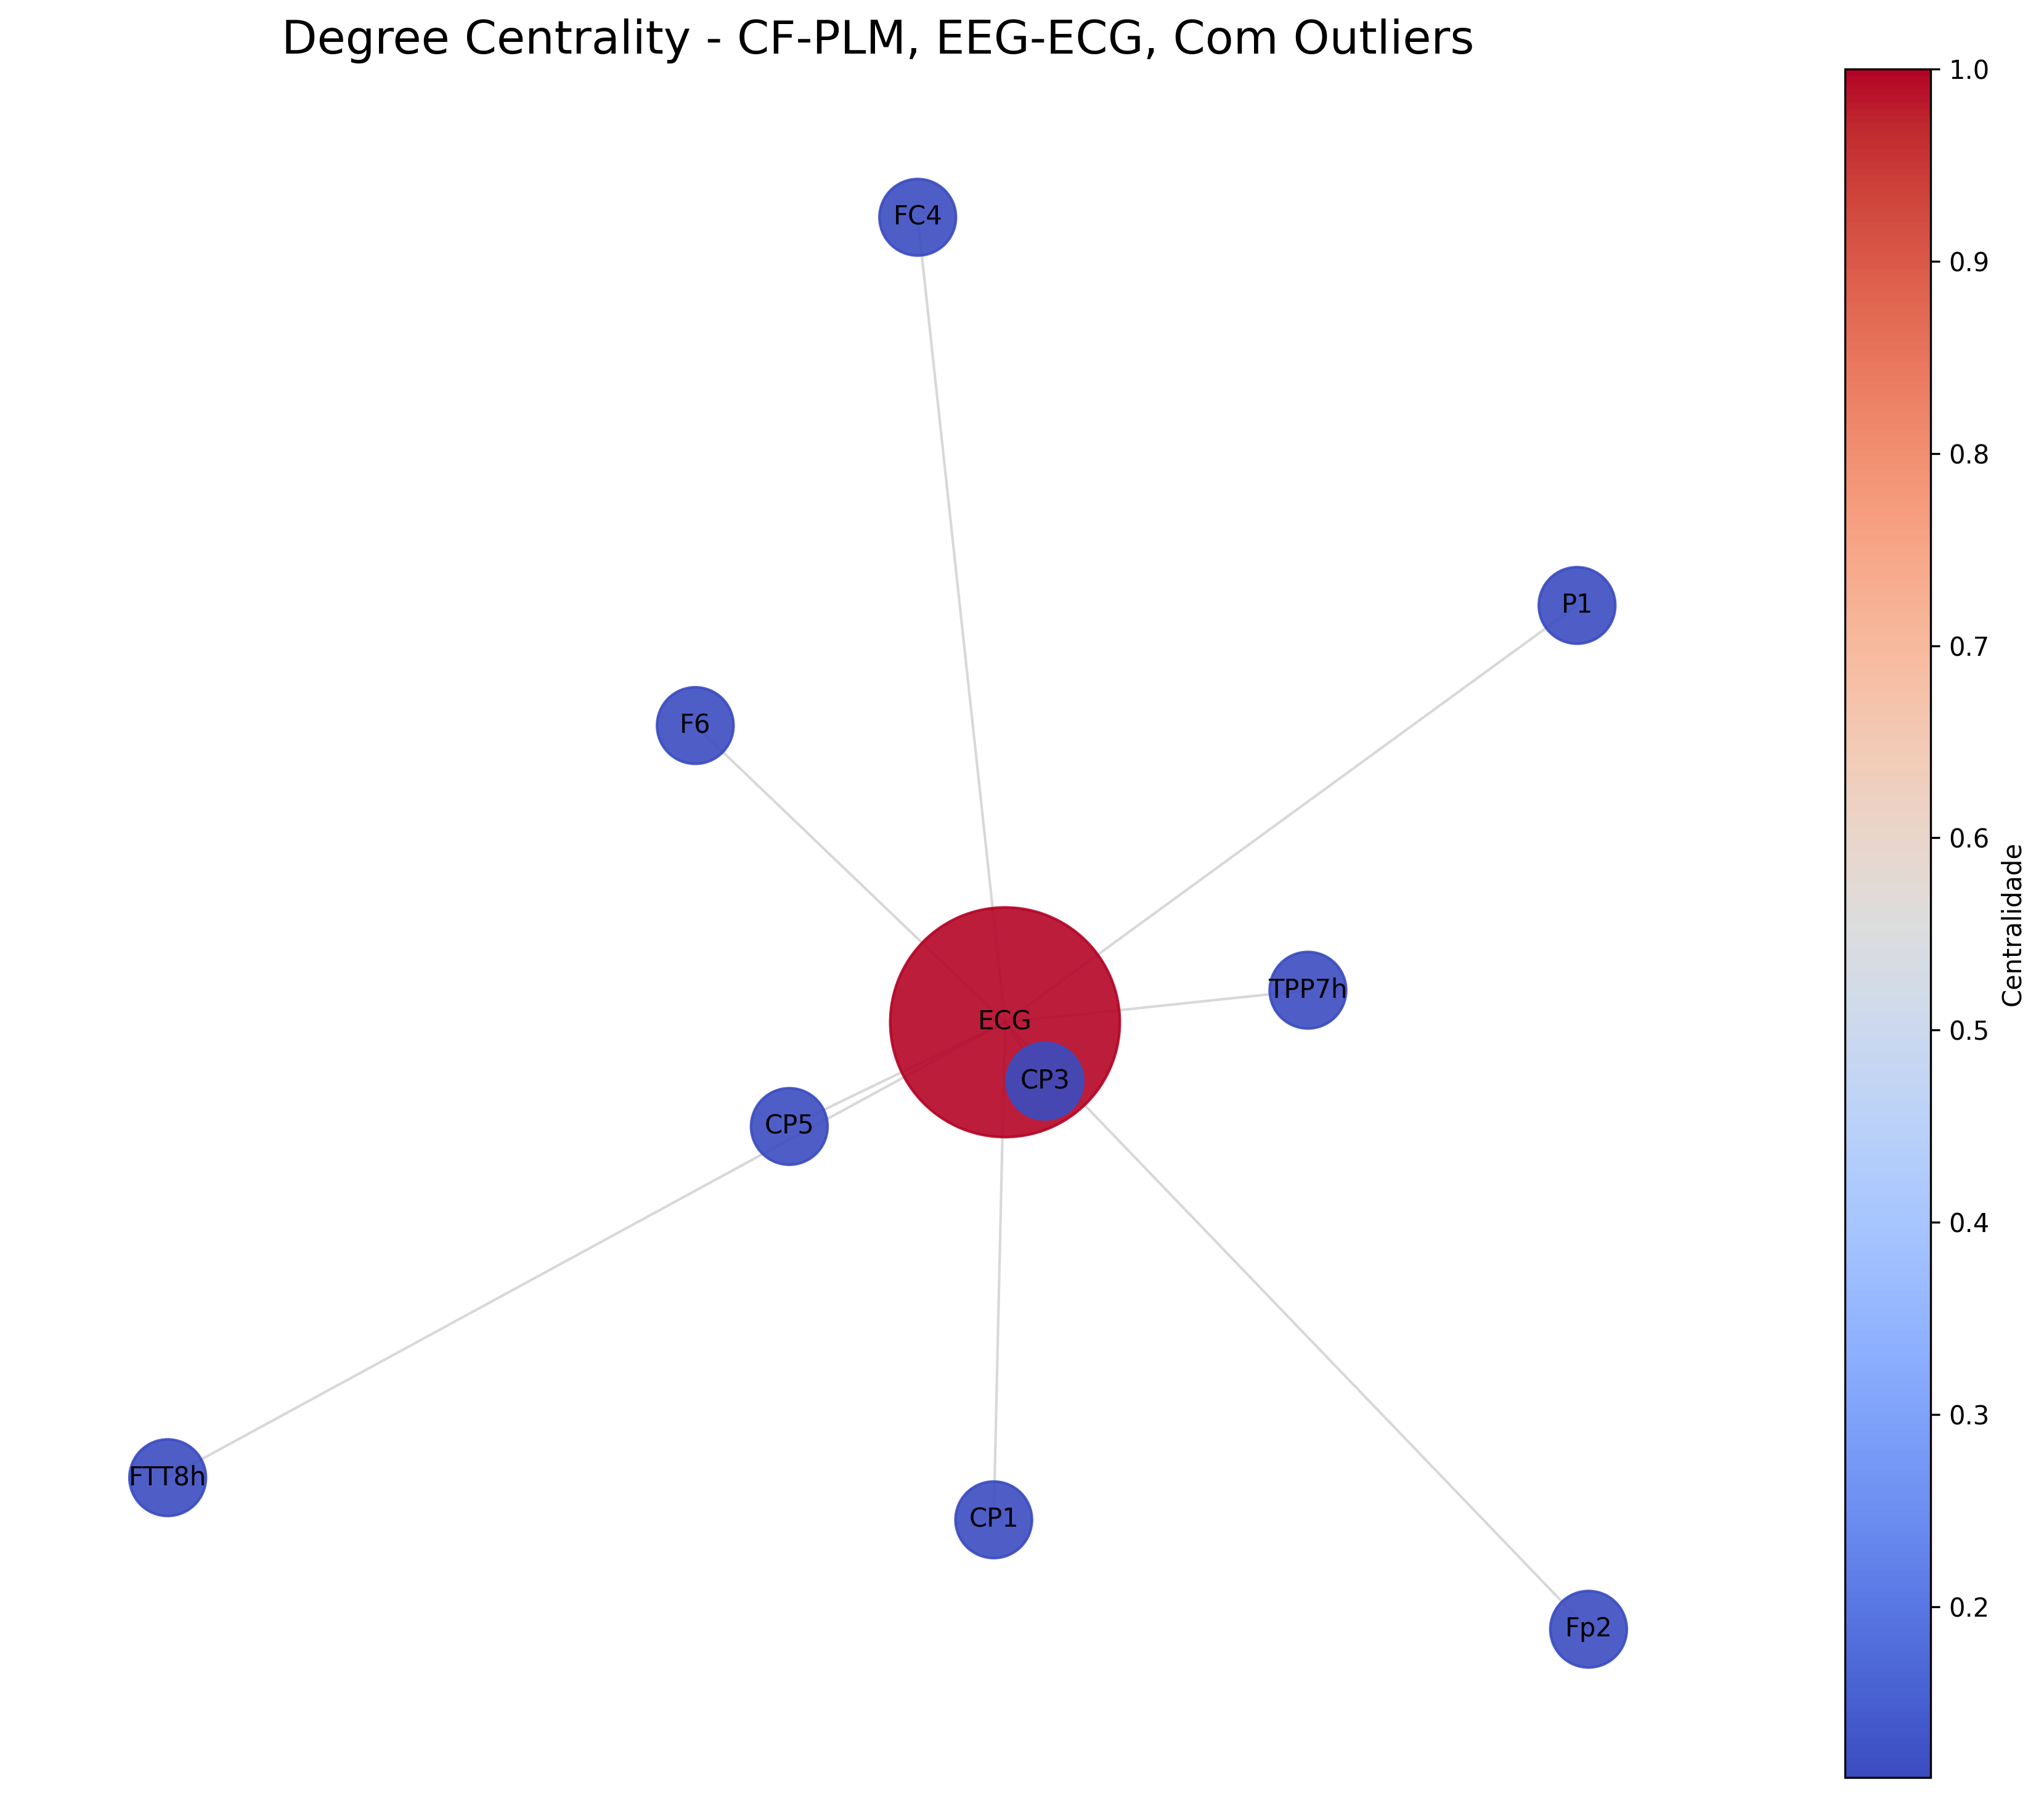
\includegraphics[width=0.45\textwidth]{figs/7_bootstrap_results_analysis/3_centrality_graphs/Degree_Centrality__CFPLM_EEGECG_Com_Outliers.png}
        \label{fig:dc_cfplm_eegecg_com}
    }
    \quad
    \subfloat[Sem Outliers]{
        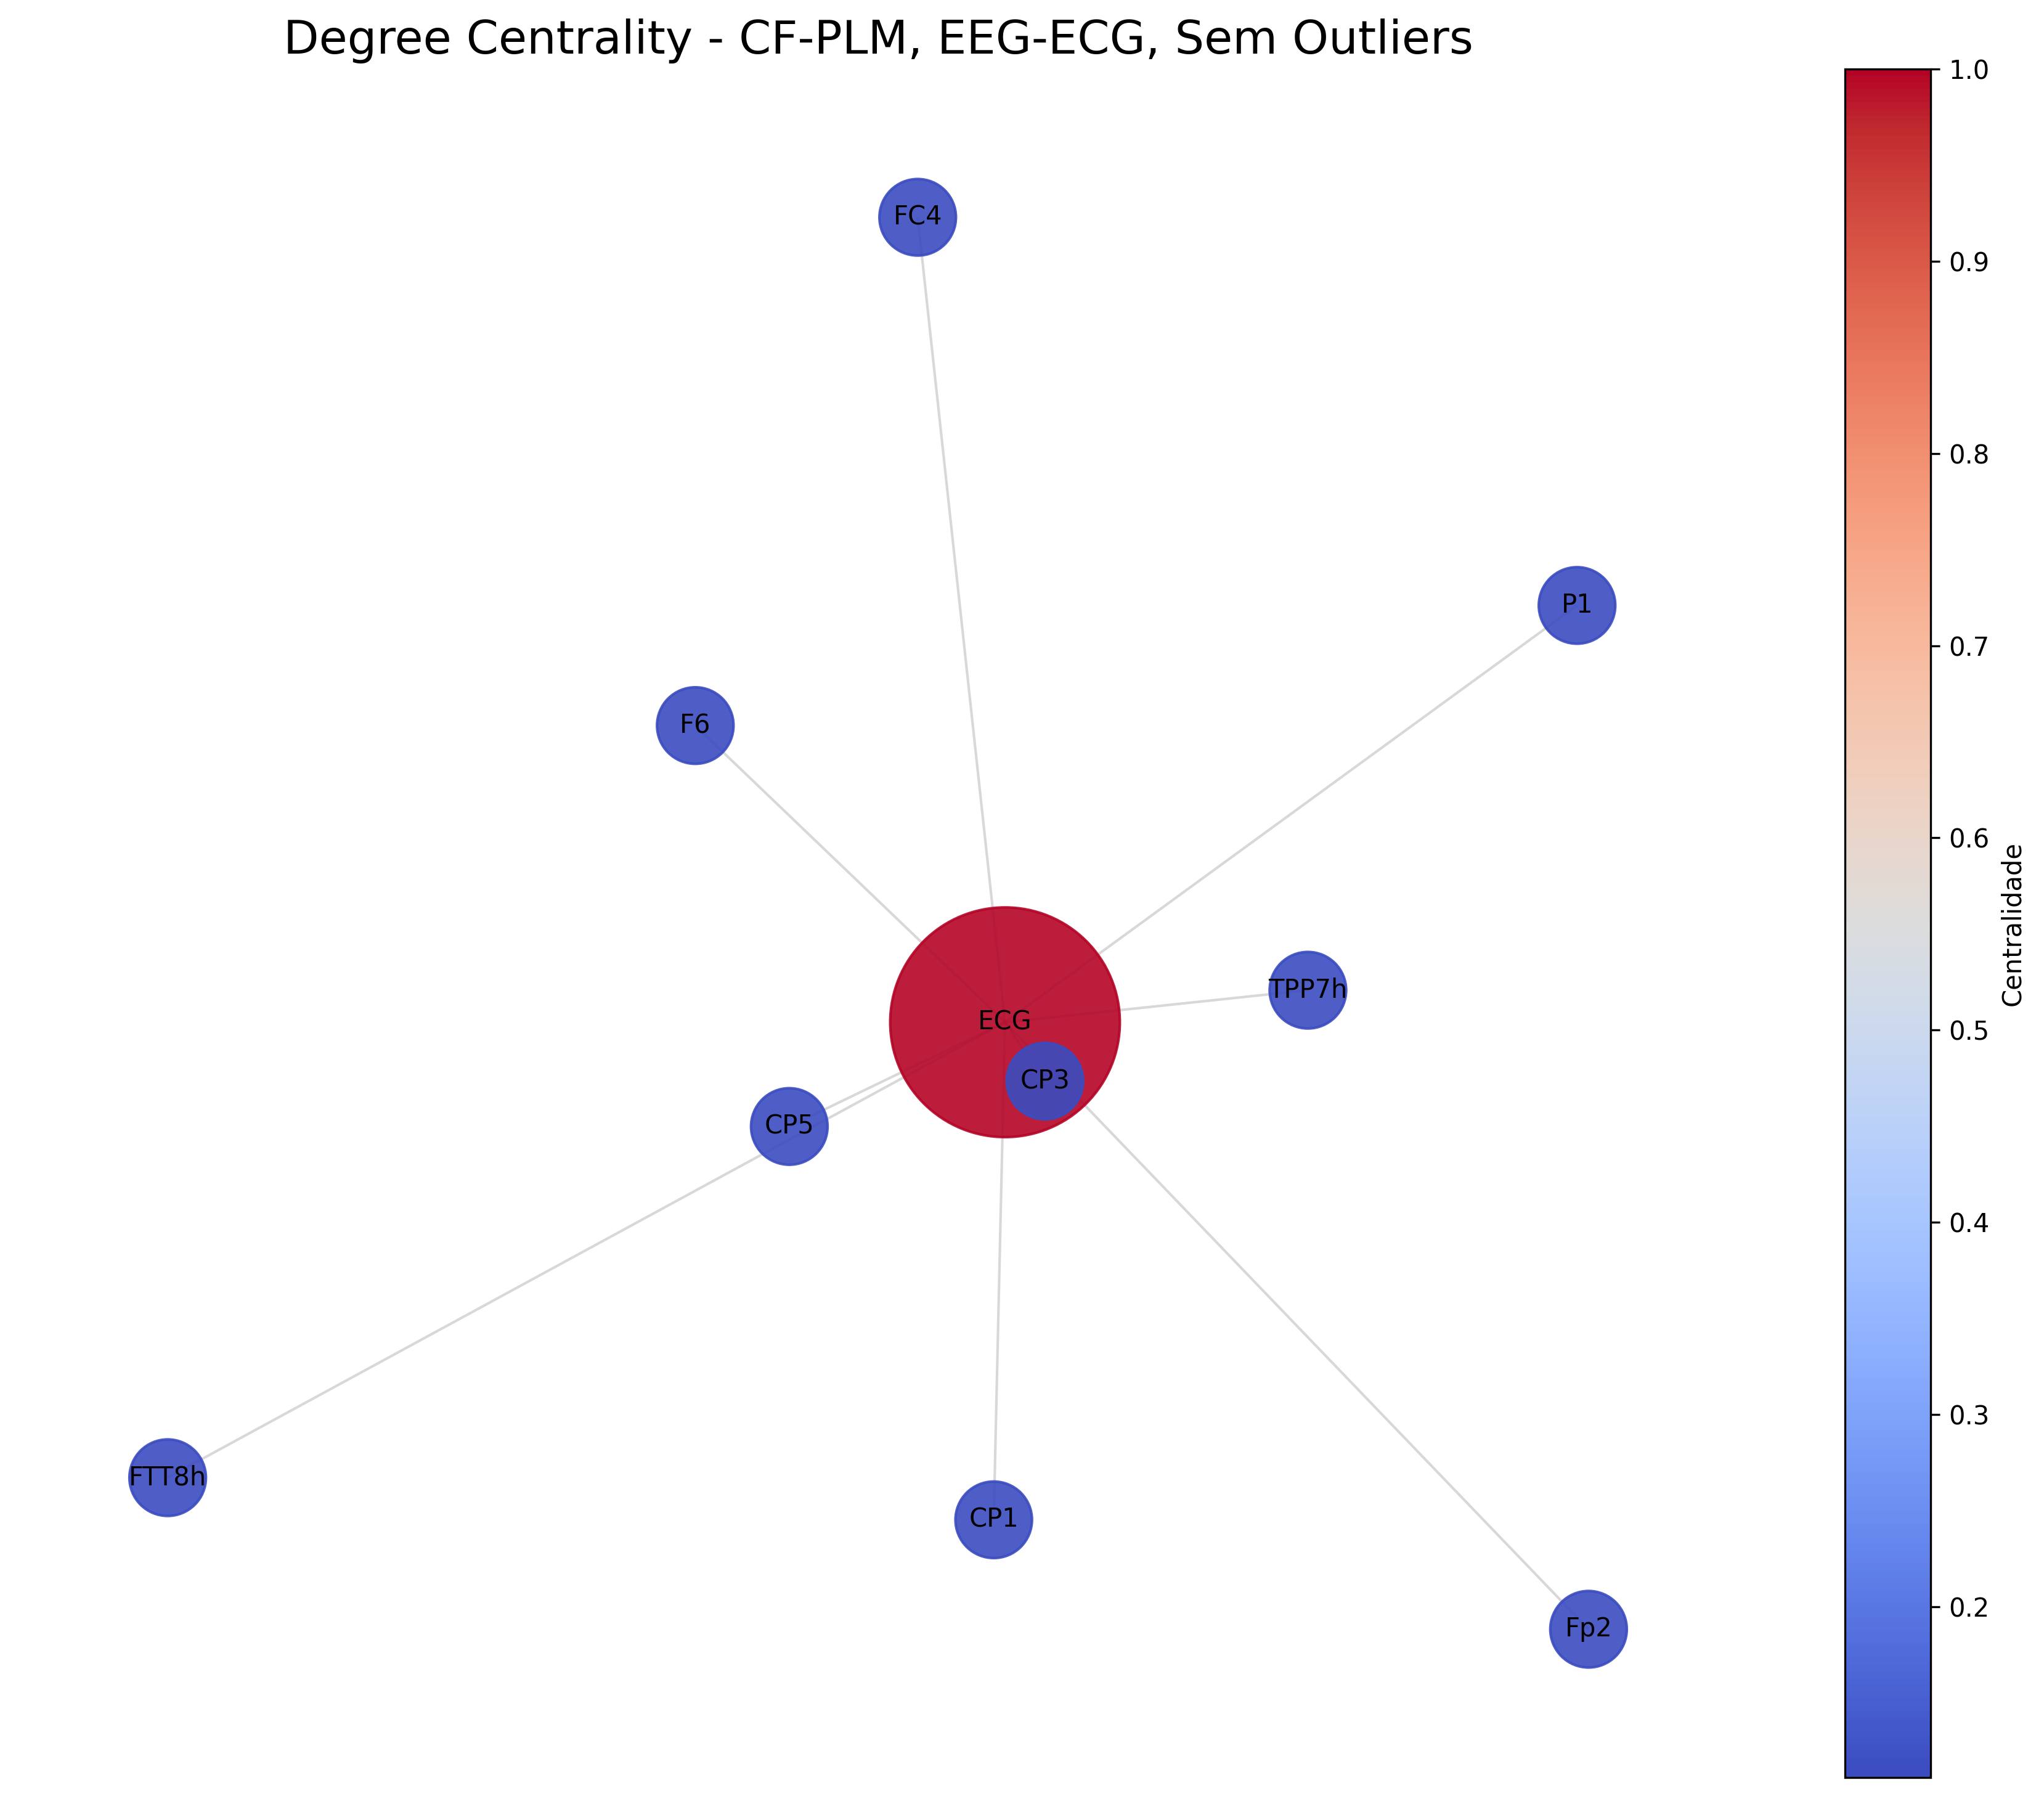
\includegraphics[width=0.45\textwidth]{figs/7_bootstrap_results_analysis/3_centrality_graphs/Degree_Centrality__CFPLM_EEGECG_Sem_Outliers.png}
        \label{fig:dc_cfplm_eegecg_sem}
    }
    \caption{Degree Centrality no cenário CF-PLM (EEG-ECG). O canal \emph{ECG} mantém o grau mais alto em ambos os cenários.}
    \label{fig:dc_cfplm_eegecg}
\end{figure}

Na Figura~\ref{fig:dc_cfplm_eegecg}, o canal \emph{ECG} domina a rede com o maior grau, pois é o único canal cardíaco e todas as conexões cross-frequency entre EEG e ECG passam por ele. Assim, todos os canais EEG conectados ao \emph{ECG} elevam seu grau, mas o \emph{ECG} concentra a maior parte das conexões diretas \cite{rubinov2010complex}. A remoção de outliers não altera essa hierarquia.

\subsubsection{PLI (EEG-EEG)}
\begin{figure}[htb]
    \centering
    \subfloat[Com Outliers]{
        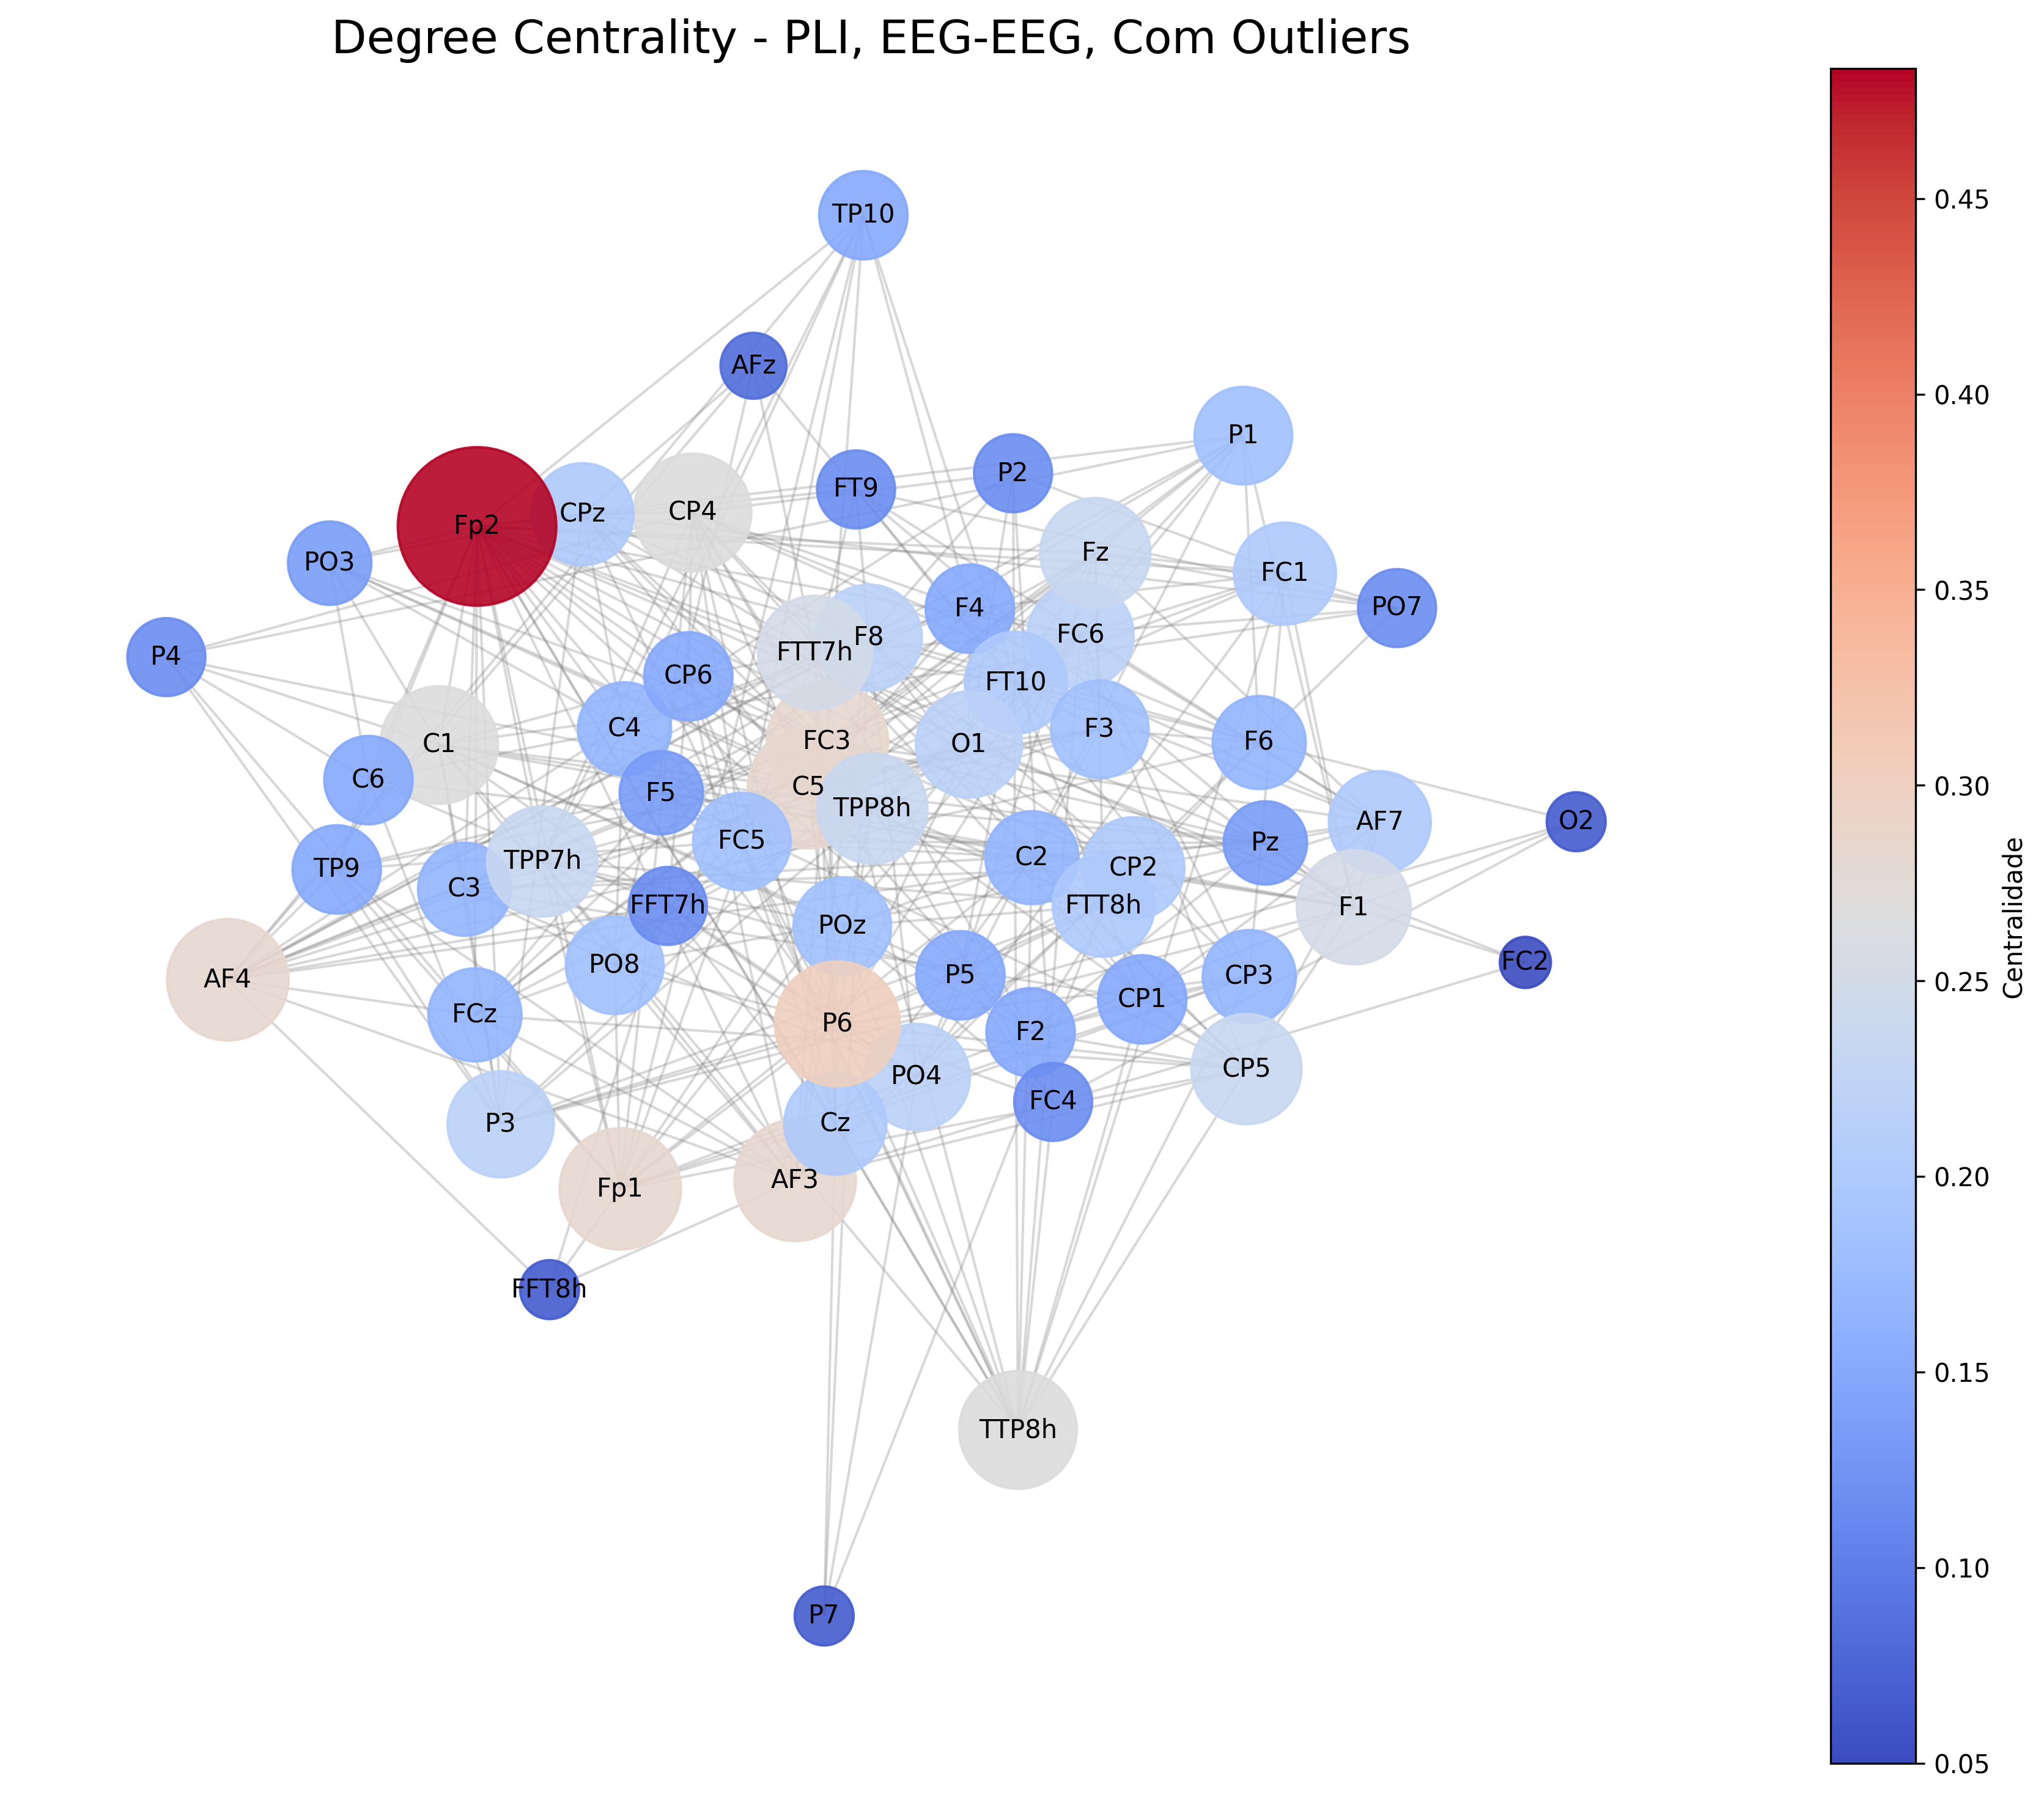
\includegraphics[width=0.45\textwidth]{figs/7_bootstrap_results_analysis/3_centrality_graphs/Degree_Centrality__PLI_EEGEEG_Com_Outliers.png}
        \label{fig:dc_pli_eegeeg_com}
    }
    \quad
    \subfloat[Sem Outliers]{
        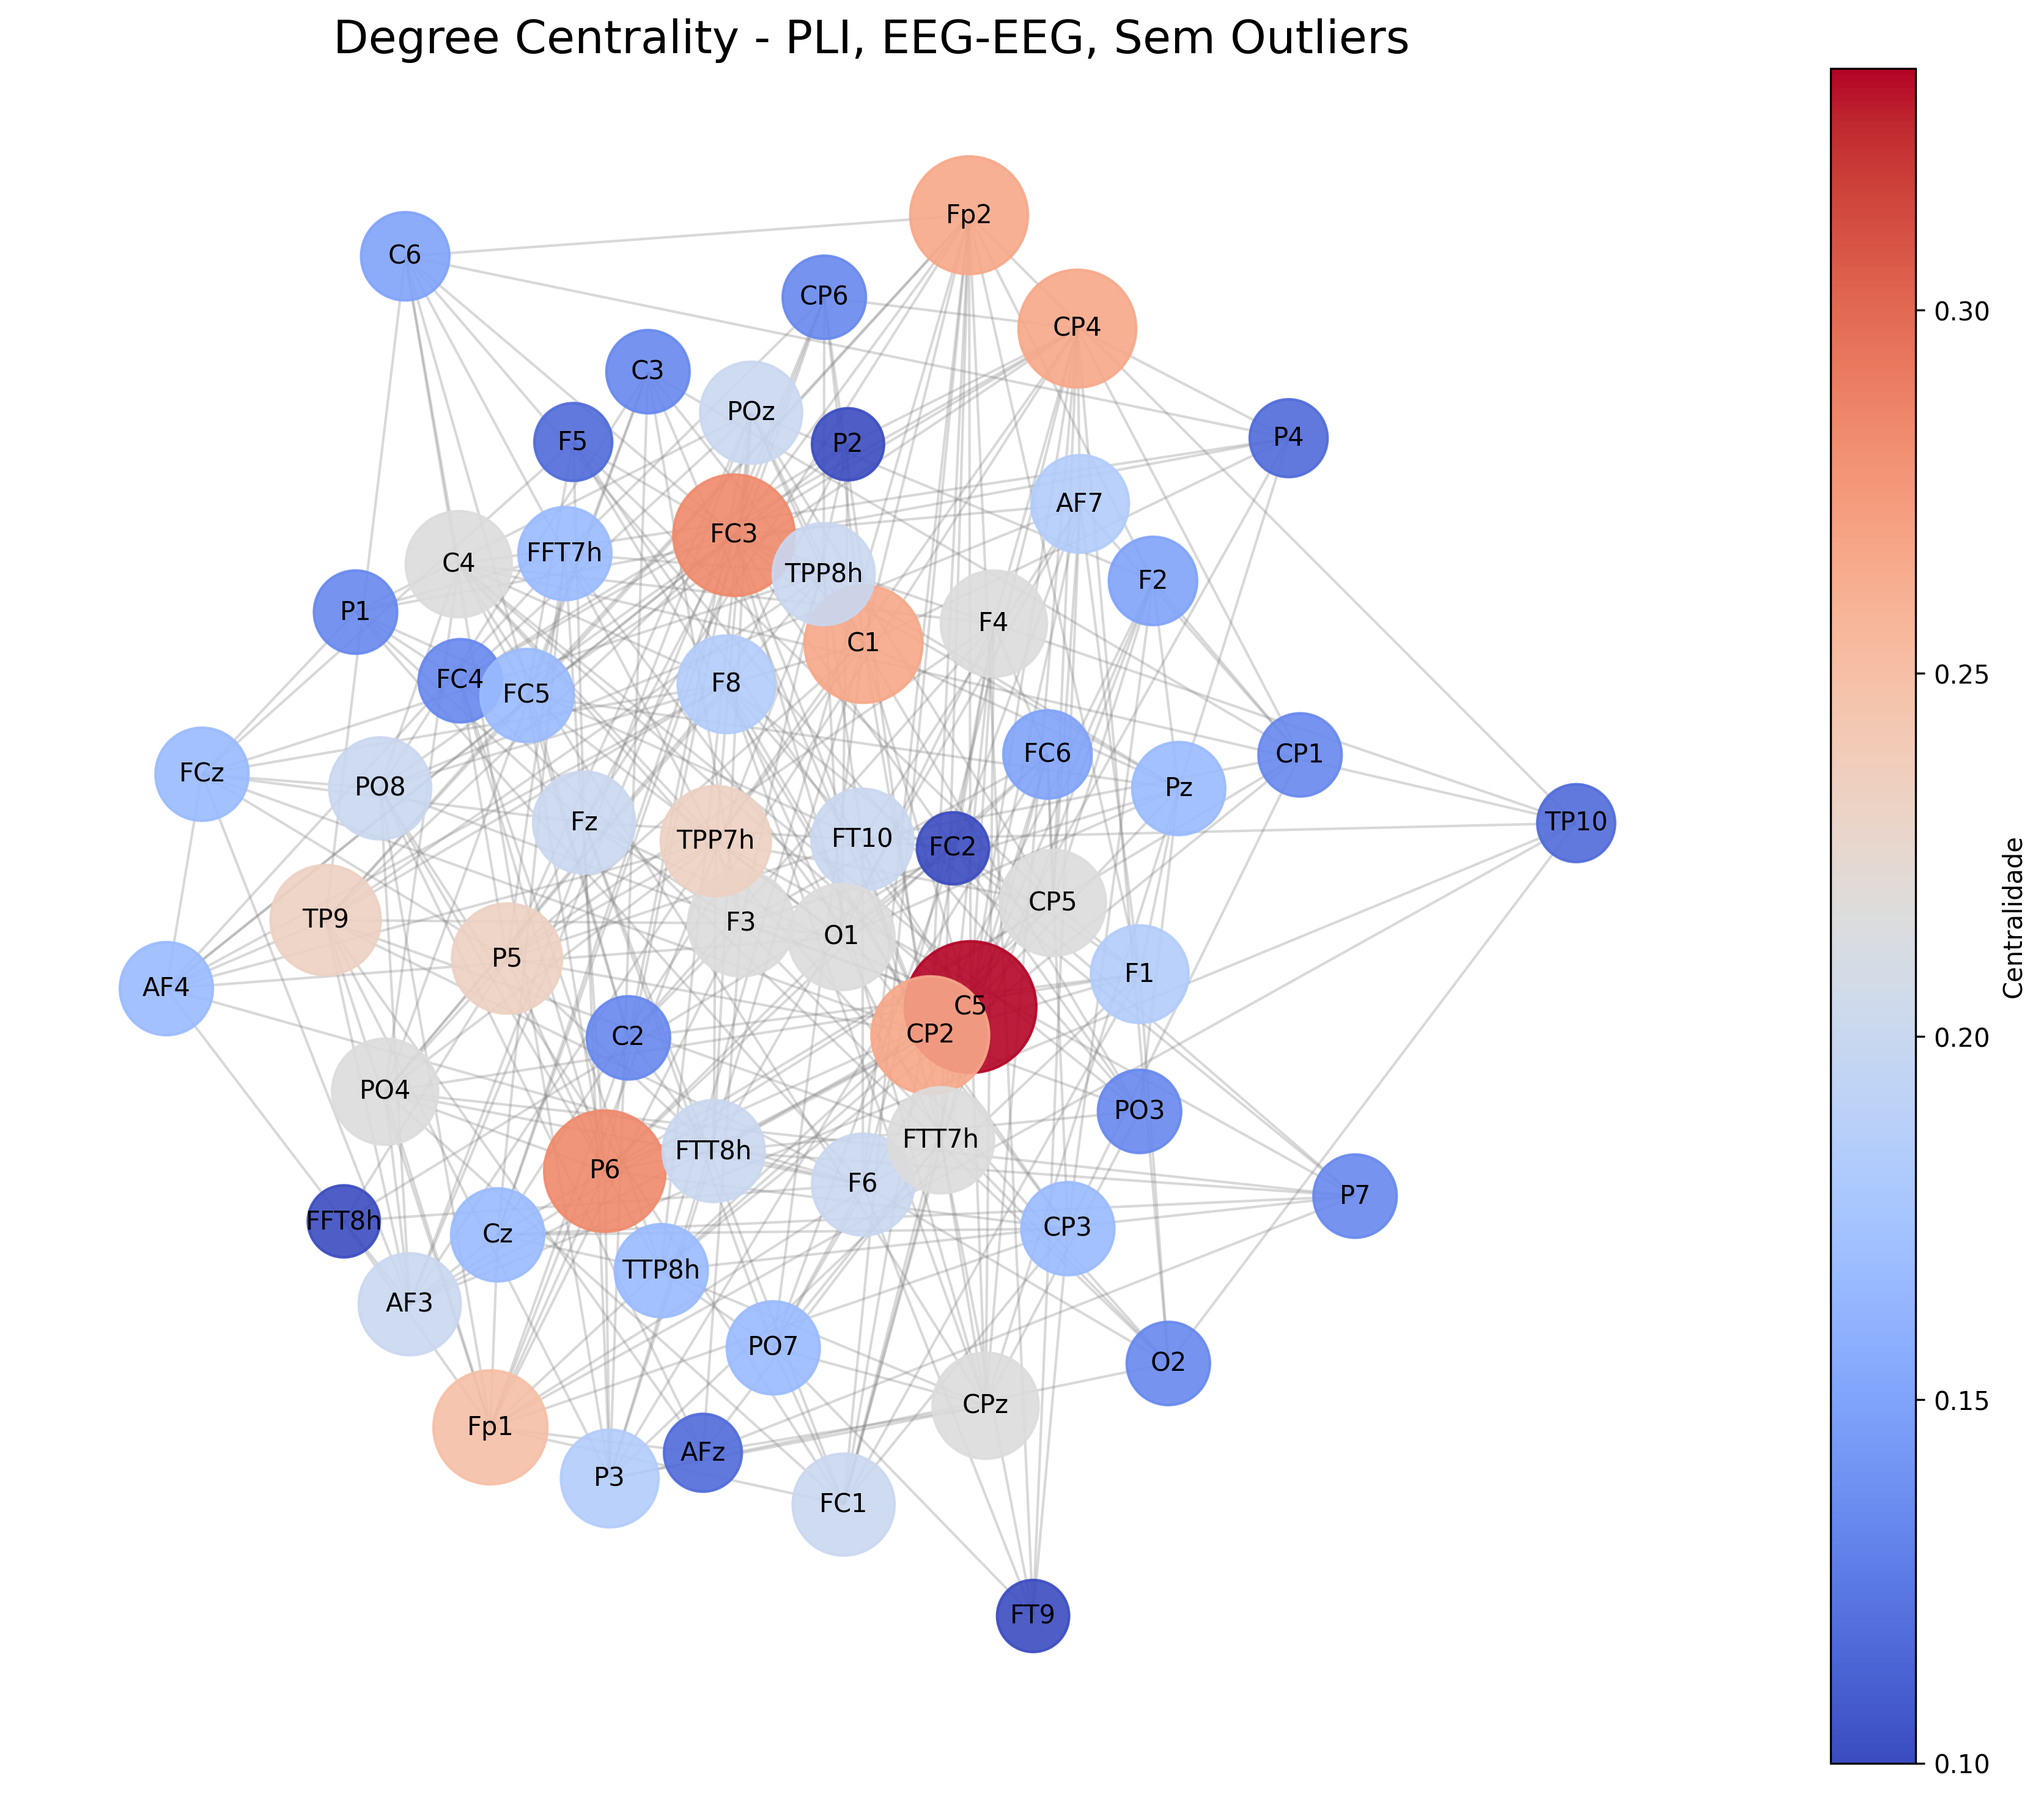
\includegraphics[width=0.45\textwidth]{figs/7_bootstrap_results_analysis/3_centrality_graphs/Degree_Centrality__PLI_EEGEEG_Sem_Outliers.png}
        \label{fig:dc_pli_eegeeg_sem}
    }
    \caption{Degree Centrality no cenário PLI (EEG-EEG). Alguns canais (por exemplo, Fp2, CP2) apresentam alto grau de conexões diretas.}
    \label{fig:dc_pli_eegeeg}
\end{figure}

Na Figura~\ref{fig:dc_pli_eegeeg}, observa-se que, no contexto de PLI (EEG-EEG), determinados canais, como Fp2 e CP2, se destacam por estabelecerem um maior número de conexões diretas de \emph{phase lag} com outros canais, sugerindo que tais canais atuam como “hubs de comunicação” \cite{newman2010networks}. A estrutura global da rede permanece inalterada no cenário sem outliers, evidenciando a robustez do padrão de conectividade.



\subsection{Eigenvector Centrality}

A \emph{eigenvector centrality} avalia a relevância de um nó com base não apenas no número de conexões diretas, mas também na importância das conexões indiretas que ele estabelece. Segundo \cite{bonacich1972factoring}, essa métrica fundamenta-se em ponderações da importância relativa dos nós, de modo que nós conectados a outros nós igualmente relevantes apresentam maior centralidade. No contexto deste estudo, a \emph{eigenvector centrality} é particularmente útil para identificar canais centrais que exercem influência tanto diretamente quanto indiretamente sobre a sincronização nas redes EEG-ECG (CF-PLM) e EEG-EEG (PLI).

A seguir, apresentamos as análises específicas para cada grupo:

\subsubsection{CF-PLM (EEG-ECG)}
\begin{figure}[htb]
    \centering
    \subfloat[Com Outliers]{
        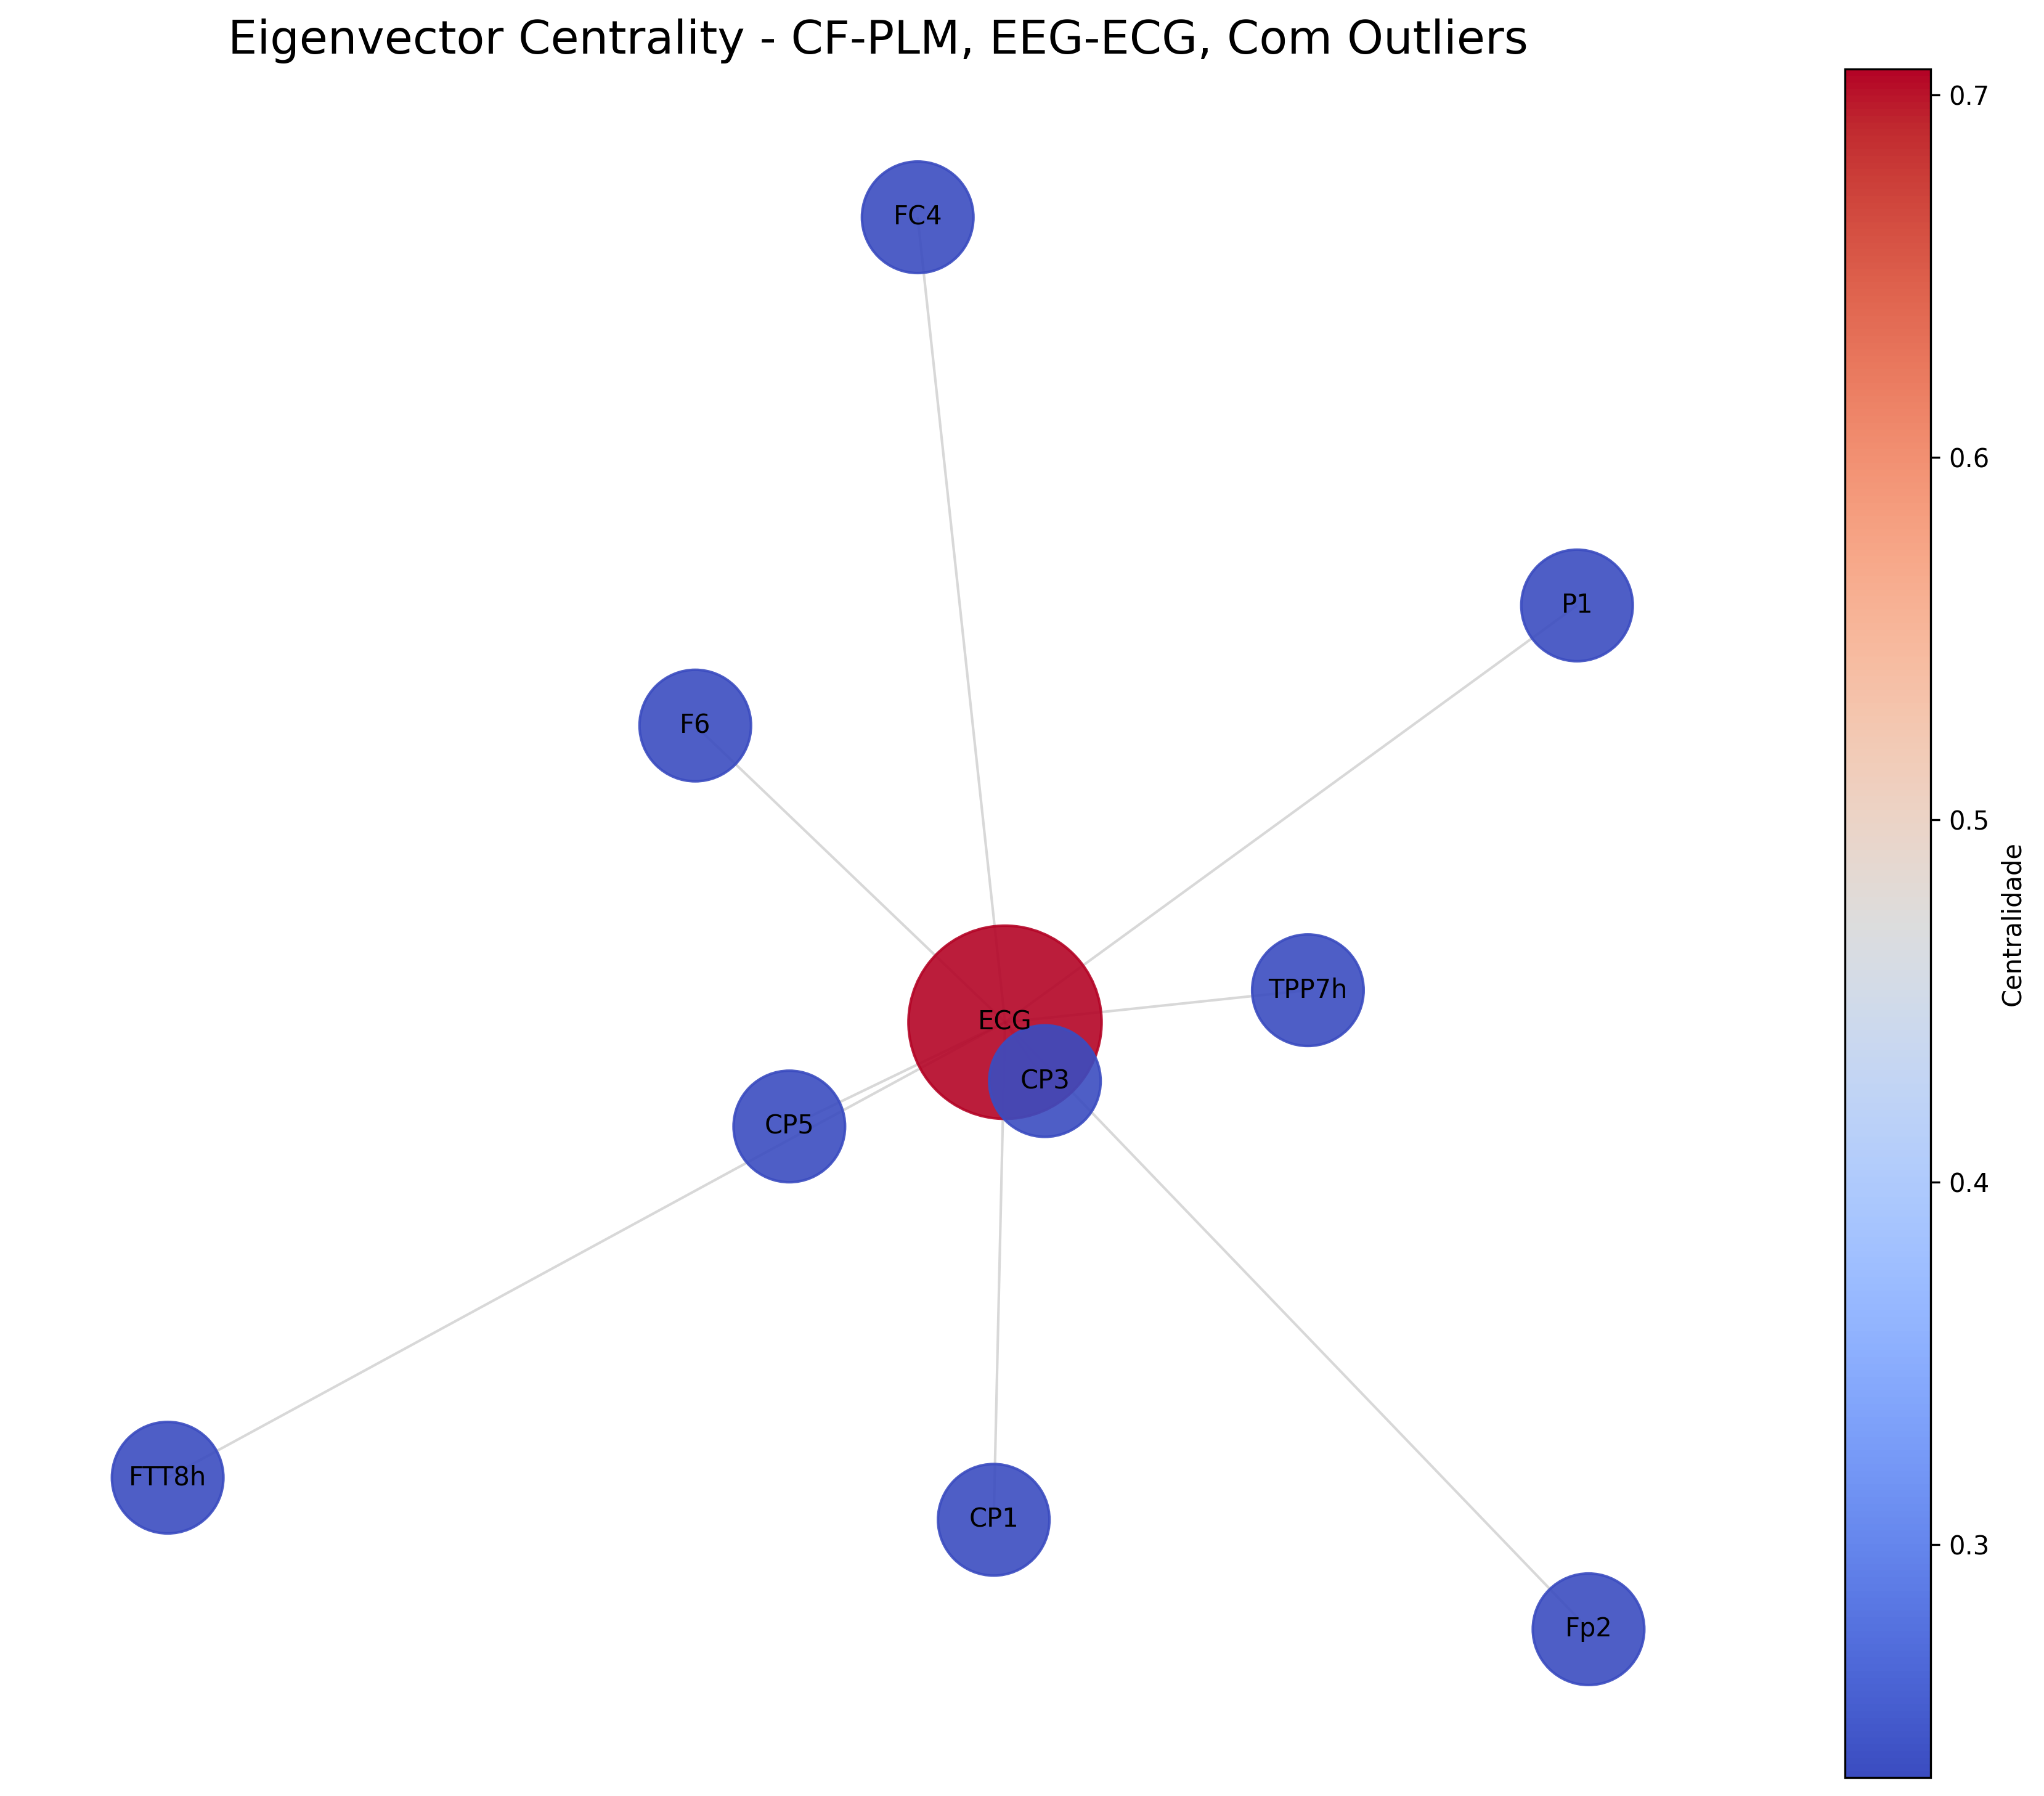
\includegraphics[width=0.45\textwidth]{figs/7_bootstrap_results_analysis/3_centrality_graphs/Eigenvector_Centrality__CFPLM_EEGECG_Com_Outliers.png}
        \label{fig:ec_cfplm_eegecg_com}
    }
    \quad
    \subfloat[Sem Outliers]{
        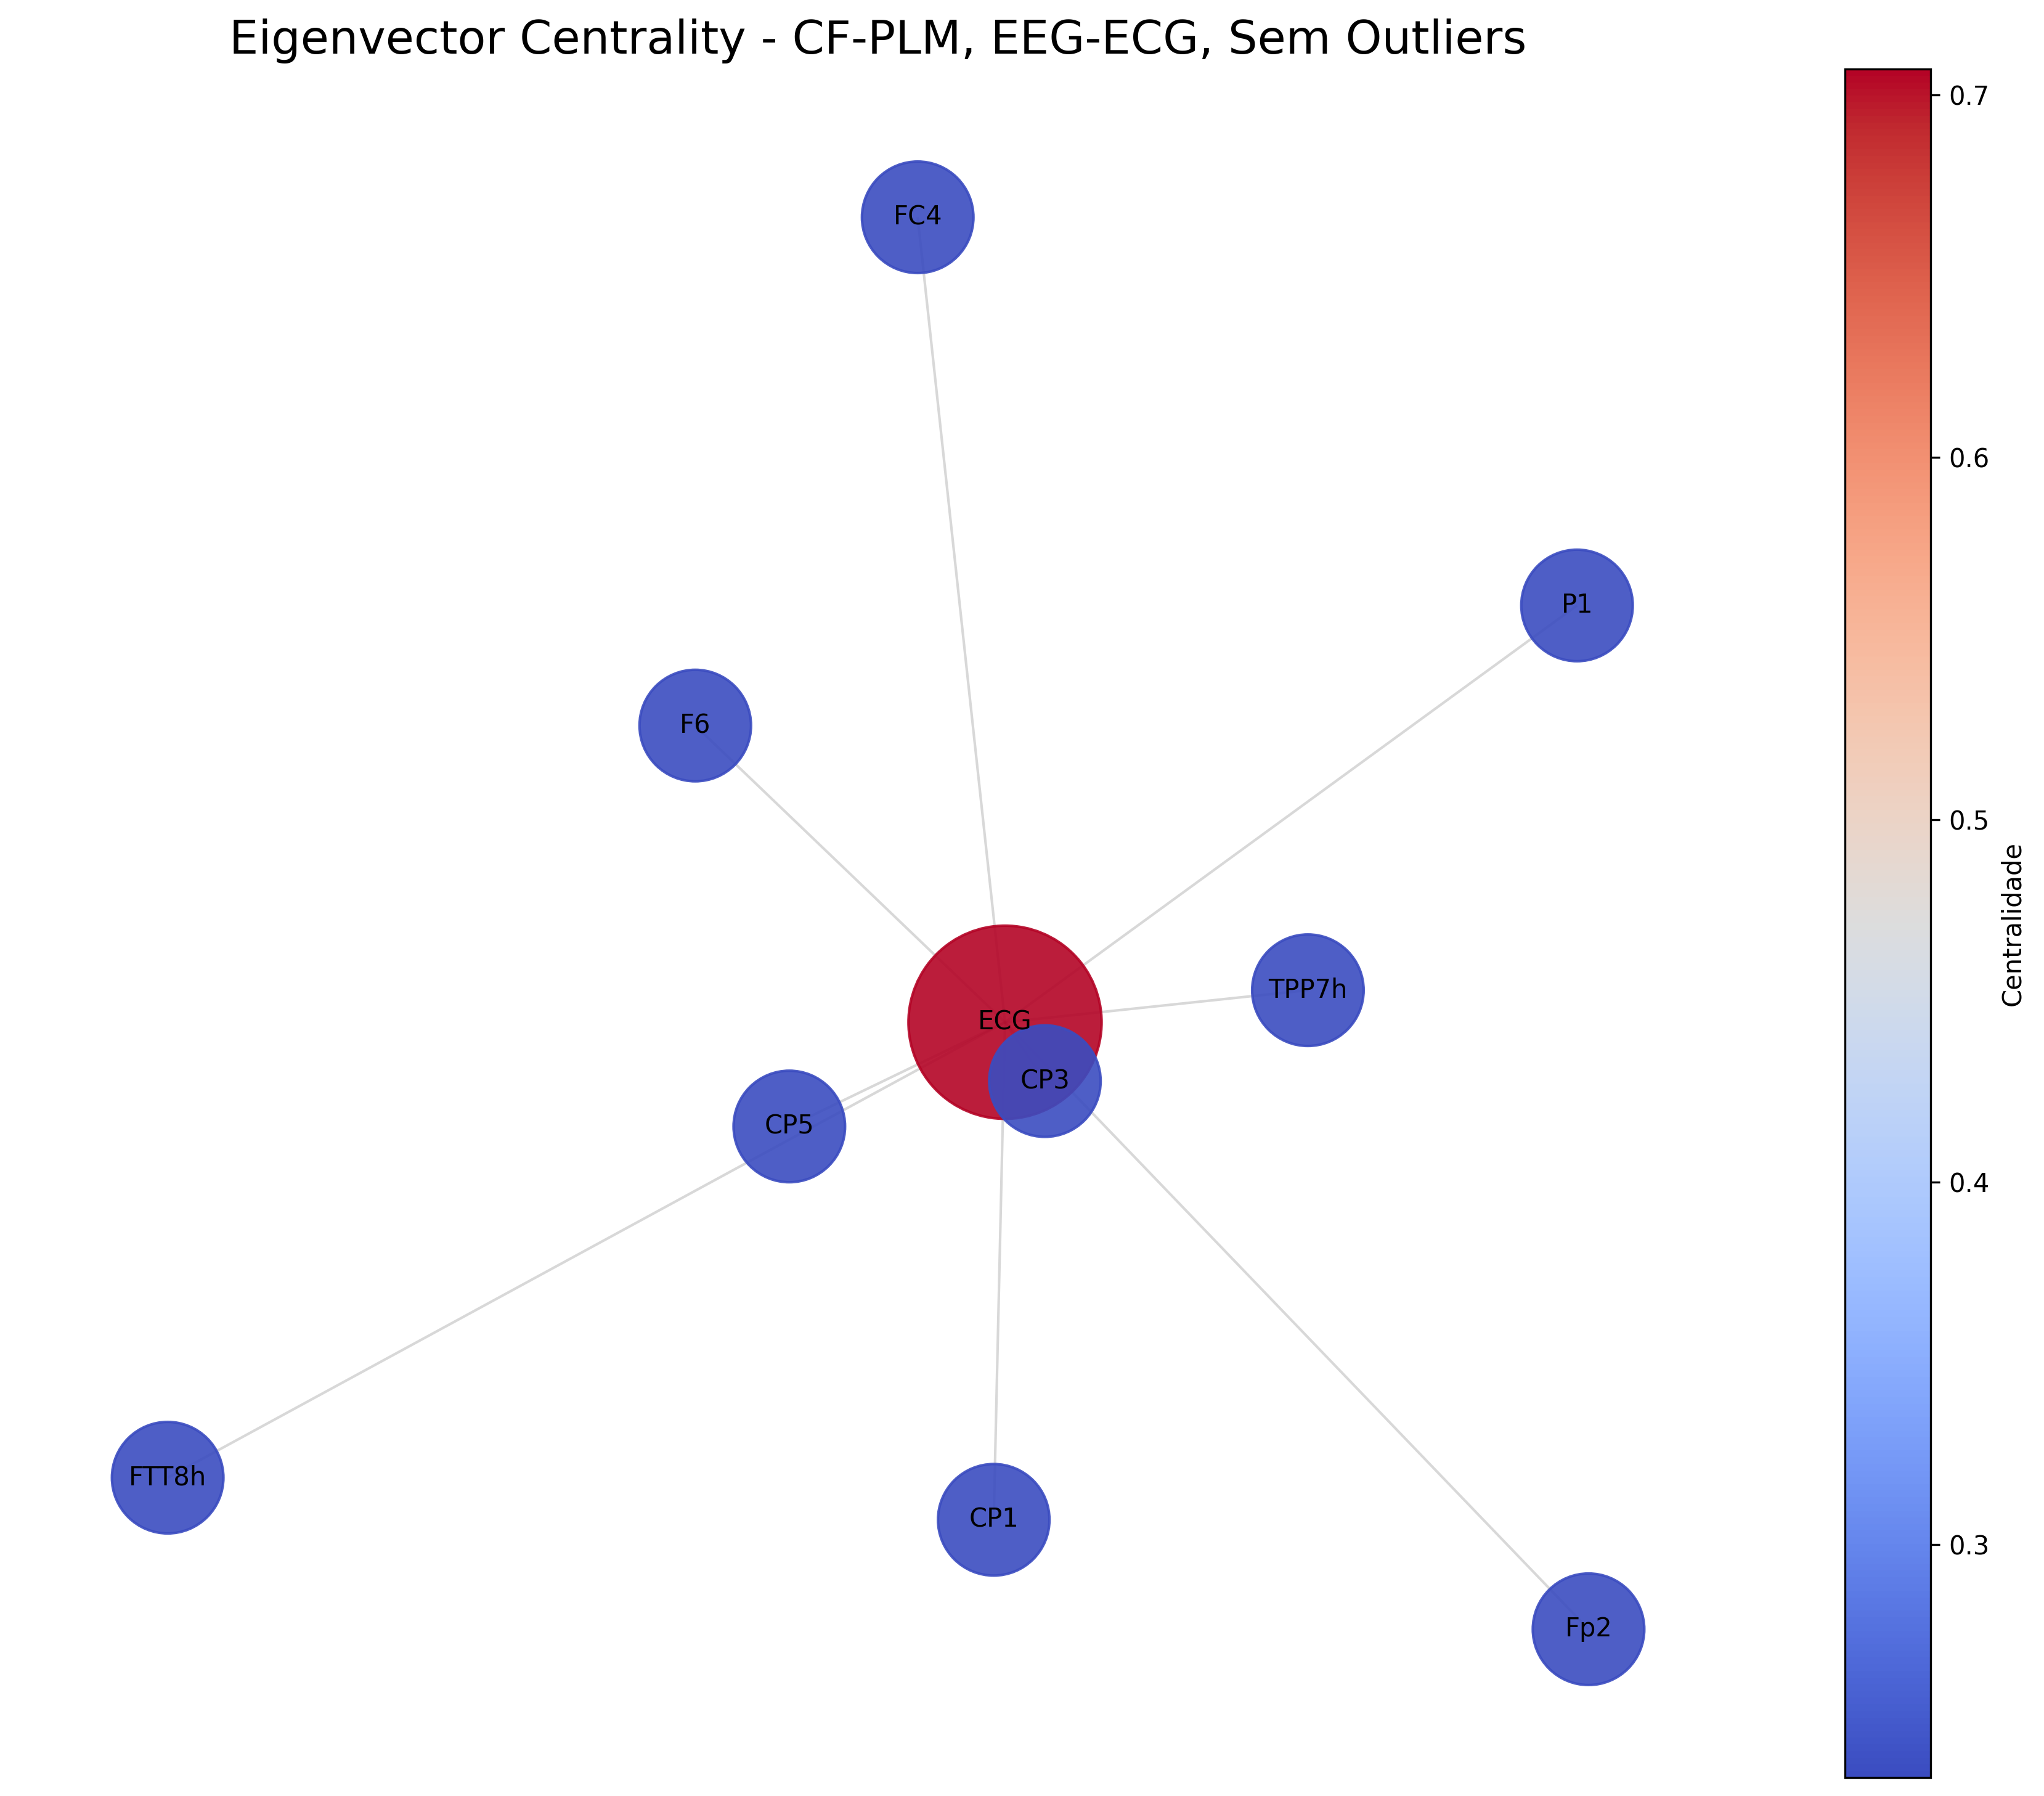
\includegraphics[width=0.45\textwidth]{figs/7_bootstrap_results_analysis/3_centrality_graphs/Eigenvector_Centrality__CFPLM_EEGECG_Sem_Outliers.png}
        \label{fig:ec_cfplm_eegecg_sem}
    }
    \caption{Eigenvector Centrality no cenário CF-PLM (EEG-ECG). O canal \emph{ECG} retém a maior centralidade em ambos os cenários.}
    \label{fig:ec_cfplm_eegecg}
\end{figure}

Na Figura~\ref{fig:ec_cfplm_eegecg}, o canal \emph{ECG} domina a \emph{eigenvector centrality} por se conectar a canais como F6 e CP5, que também apresentam relevância na rede. A remoção de outliers não altera essa predominância, confirmando a importância do canal cardíaco no acoplamento cross-frequency, conforme evidenciado por \cite{bullmore2009complex}.

\subsubsection{PLI (EEG-EEG)}
\begin{figure}[htb]
    \centering
    \subfloat[Com Outliers]{
        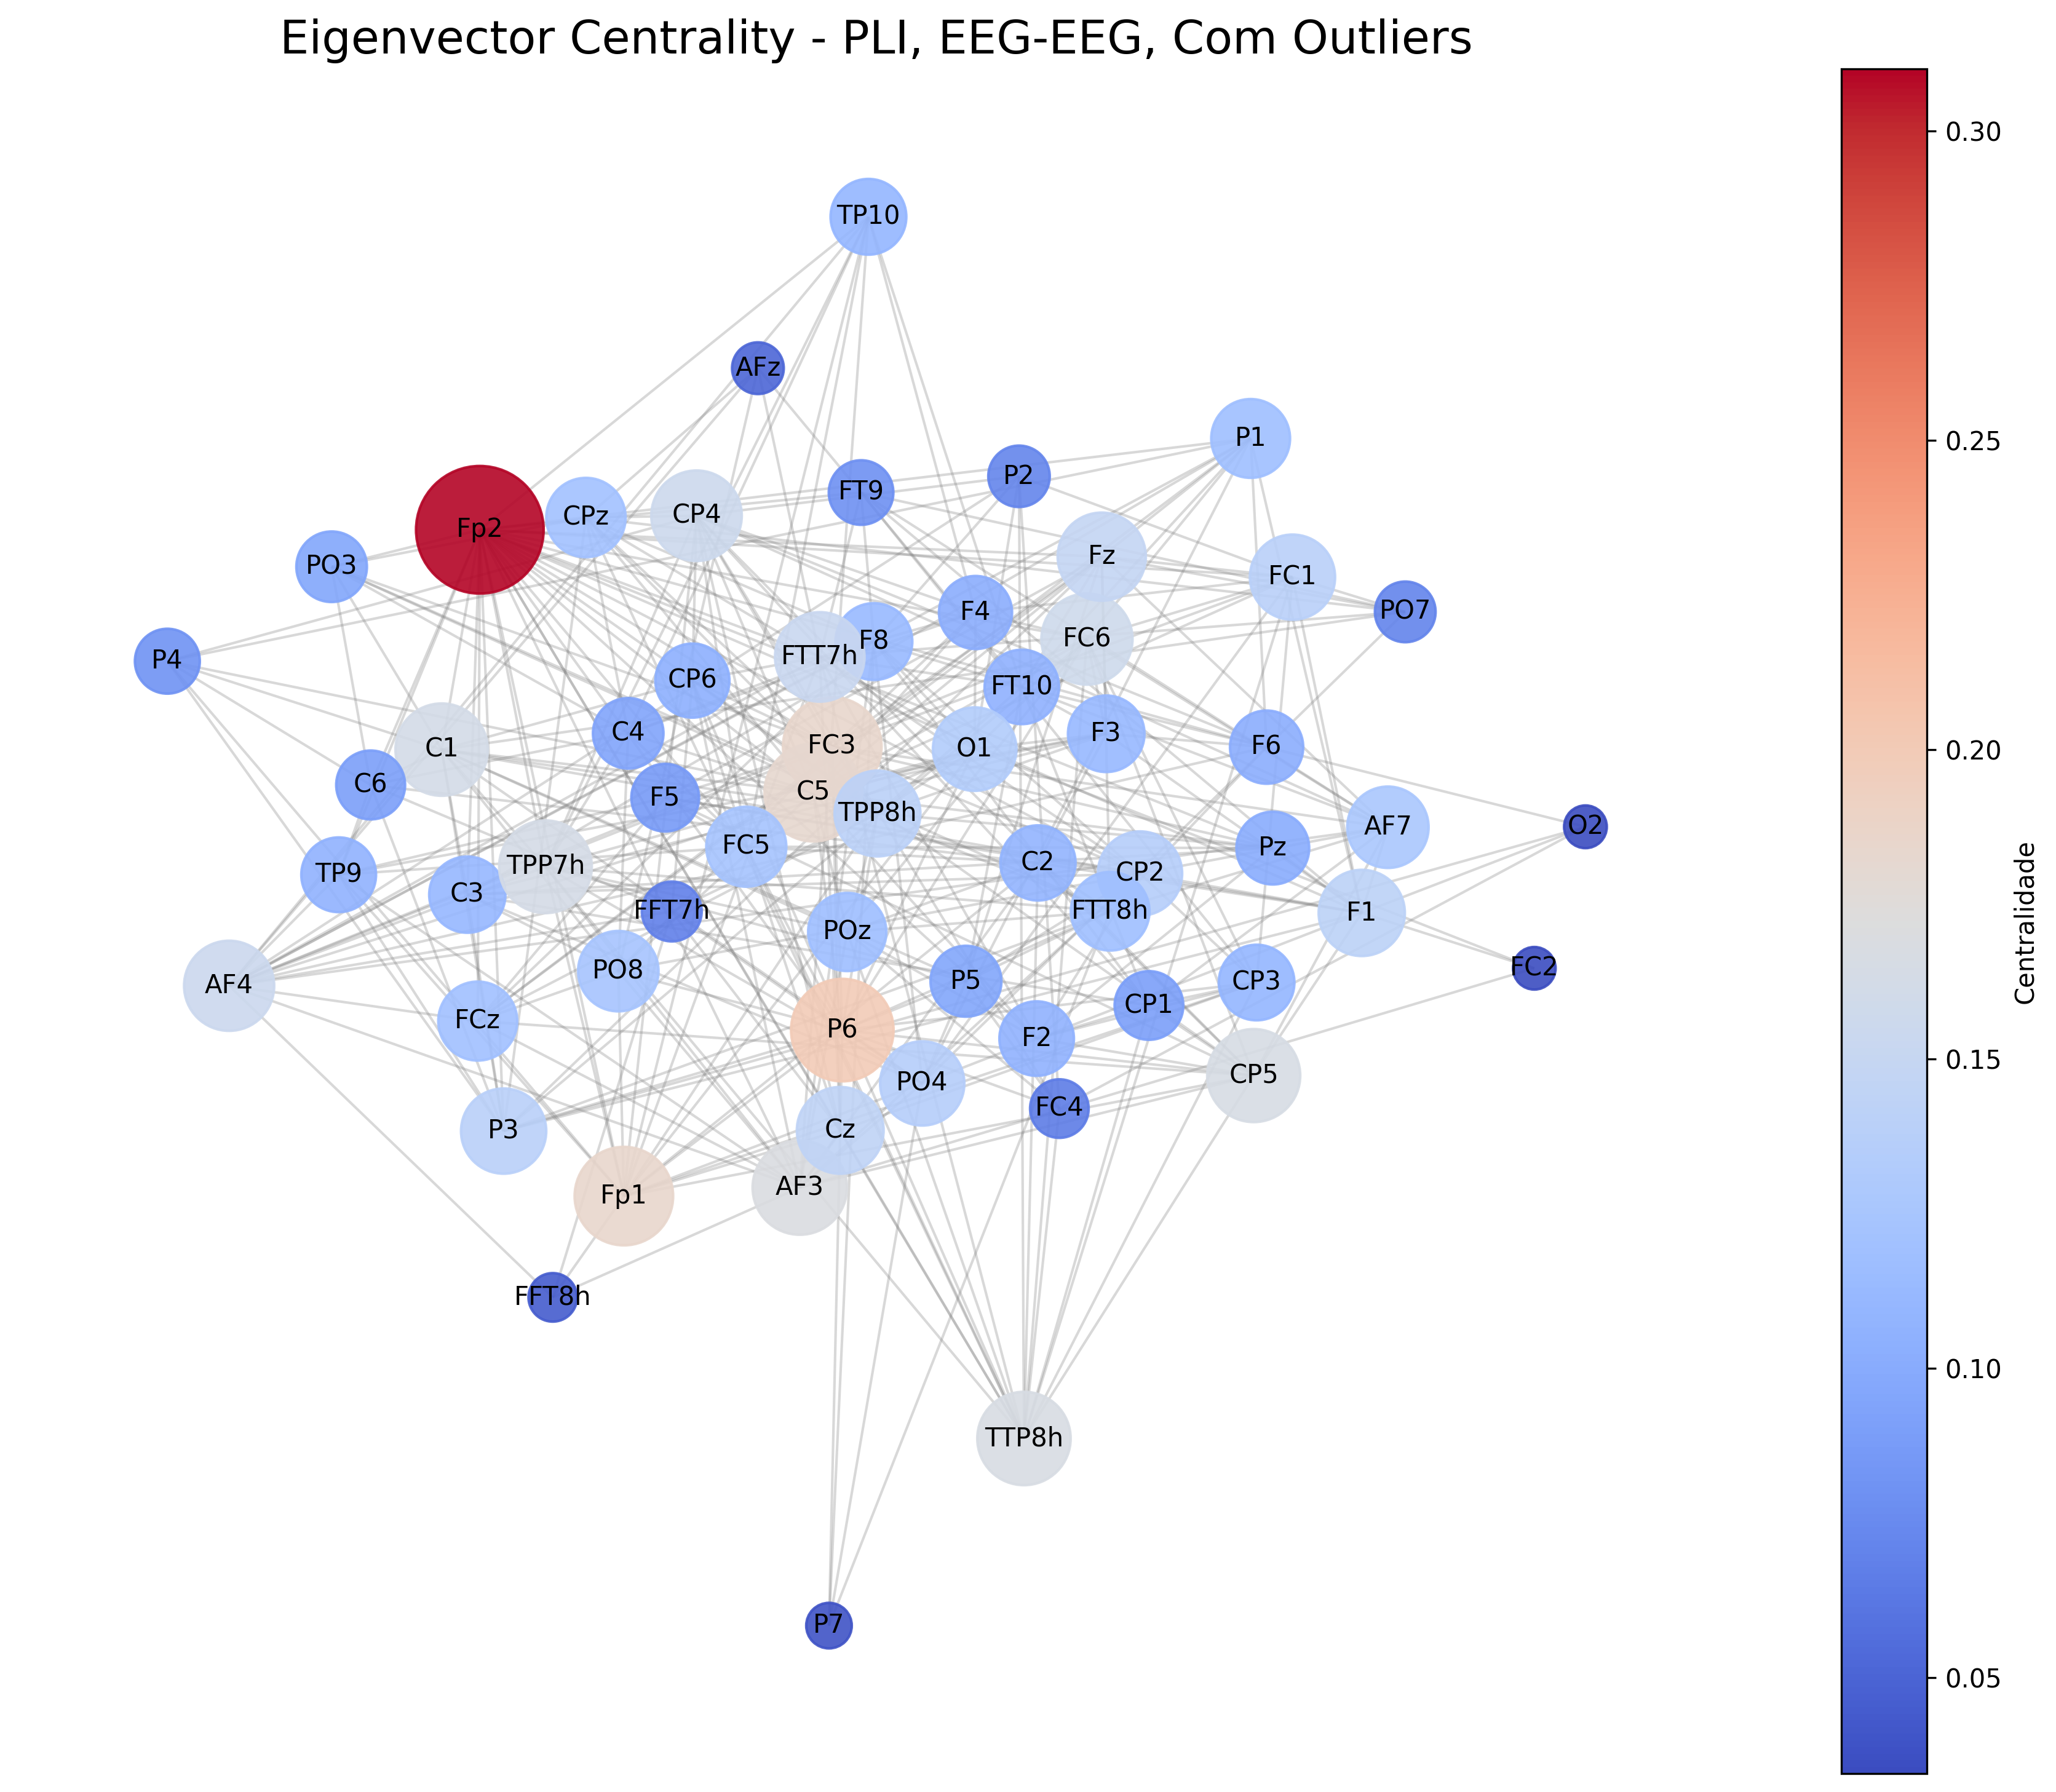
\includegraphics[width=0.45\textwidth]{figs/7_bootstrap_results_analysis/3_centrality_graphs/Eigenvector_Centrality__PLI_EEGEEG_Com_Outliers.png}
        \label{fig:ec_pli_eegeeg_com}
    }
    \quad
    \subfloat[Sem Outliers]{
        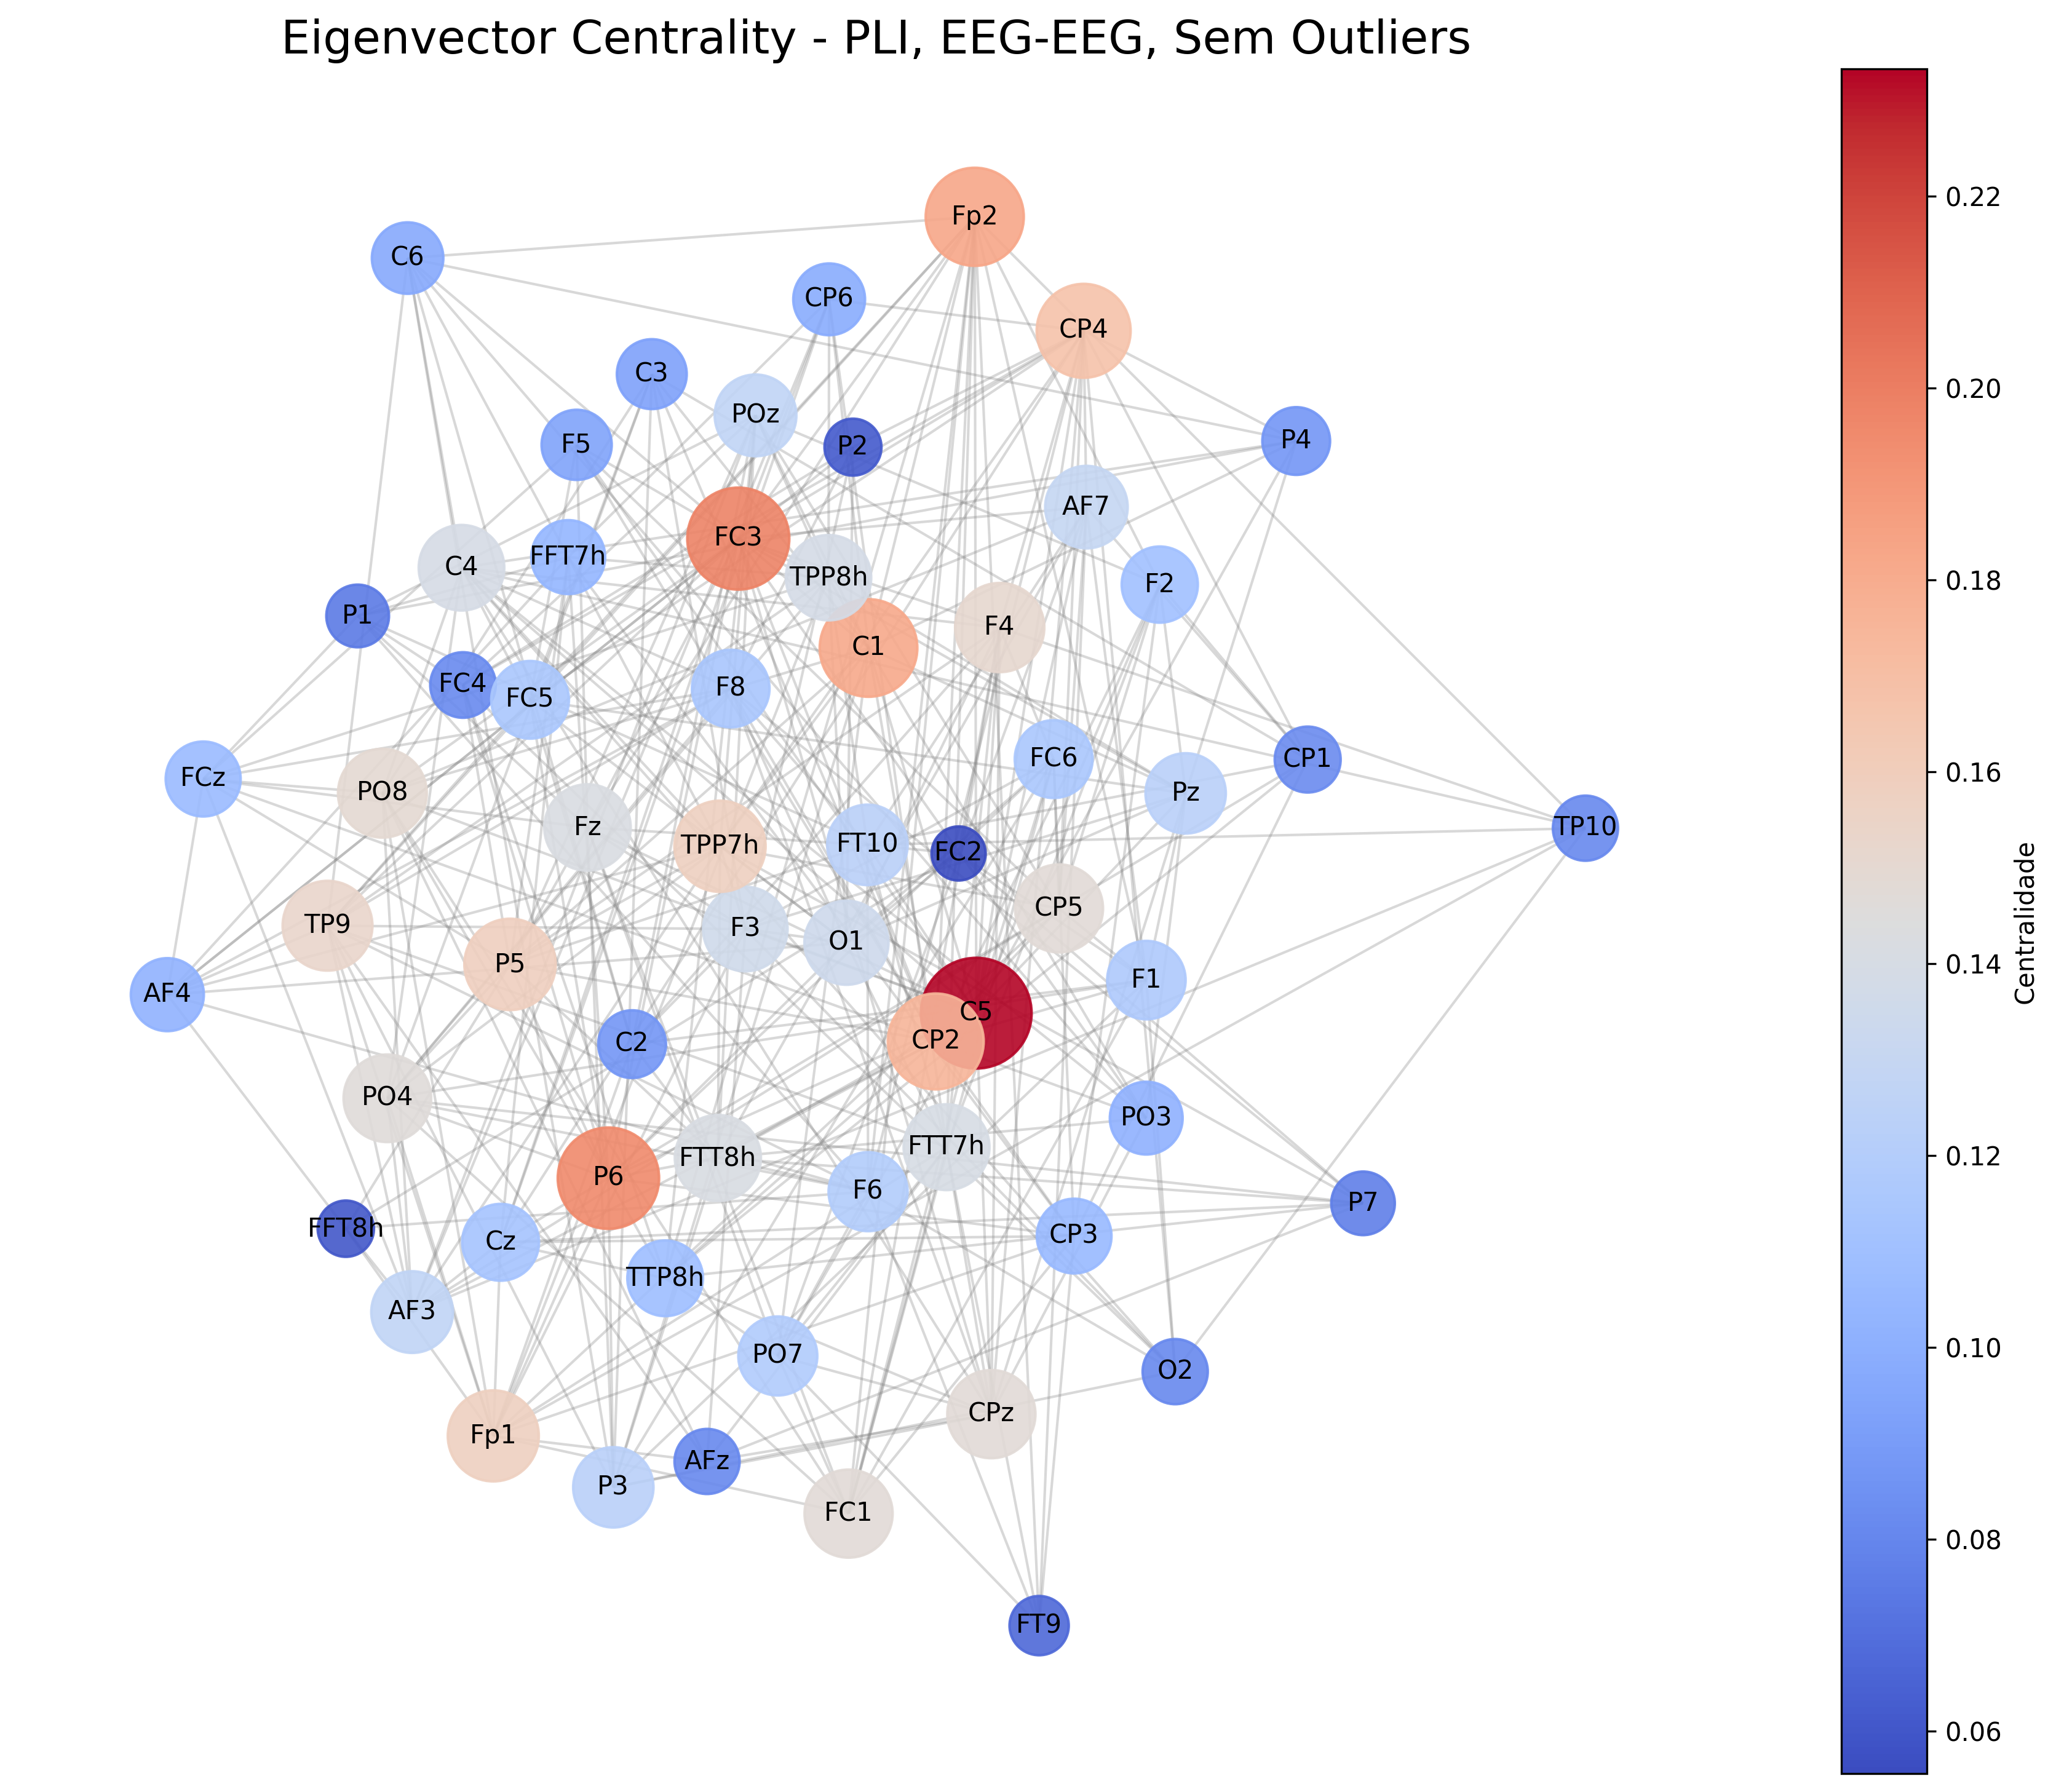
\includegraphics[width=0.45\textwidth]{figs/7_bootstrap_results_analysis/3_centrality_graphs/Eigenvector_Centrality__PLI_EEGEEG_Sem_Outliers.png}
        \label{fig:ec_pli_eegeeg_sem}
    }
    \caption{Eigenvector Centrality no cenário PLI (EEG-EEG). Alguns canais, como Fp2, CP2 e P6, emergem como nós de alta centralidade ao se conectarem com outros nós relevantes.}
    \label{fig:ec_pli_eegeeg}
\end{figure}

Na Figura~\ref{fig:ec_pli_eegeeg}, observa-se que determinados canais, como Fp2, CP2 ou P6 (dependendo da banda), se destacam na \emph{eigenvector centrality} devido à combinação de um alto número de conexões diretas e à conexão com outros nós centrais. A análise no cenário sem outliers mantém a mesma hierarquia, reforçando a robustez dos padrões de conectividade identificados.

Em resumo, a análise da \emph{eigenvector centrality} evidencia que, tanto na rede EEG-ECG quanto na rede EEG-EEG, os canais que se conectam com outros nós de alta relevância desempenham papéis centrais, o que corrobora os achados apresentados nas análises de \emph{betweenness} e \emph{degree centrality}.

\subsection{Discussão e Comparação das Métricas de Centralidade}
\label{subsec:discuss_centrality_metrics}

Cada métrica de centralidade fornece informações complementares sobre a estrutura funcional das redes, contribuindo para uma compreensão detalhada dos mecanismos de comunicação cerebral e cerebro-cardíaca:

\begin{itemize}
    \item \textbf{Betweenness Centrality:} Identifica os canais que atuam como pontes críticas no fluxo de informação, facilitando a comunicação indireta na rede \cite{freeman1977set}.
    \item \textbf{Degree Centrality:} Permite determinar rapidamente os hubs mais populares, contabilizando o número de conexões diretas de cada nó \cite{newman2010networks}.
    \item \textbf{Eigenvector Centrality:} Avalia a importância dos nós considerando não apenas as conexões diretas, mas também a relevância dos nós aos quais estão conectados \cite{bonacich1972factoring}.
\end{itemize}

\paragraph{Relações Observadas e Implicações para o Estudo}  
As métricas analisadas corroboram os achados sobre sincronização e conectividade:
\begin{itemize}
    \item Na rede EEG-ECG (CF-PLM), o canal \emph{ECG} atua consistentemente como o principal hub, devido à sua natureza de interligar os sinais de ECG com os de EEG.
    \item Na rede EEG-EEG (PLI), regiões específicas, principalmente frontais e parietais (por exemplo, Fp2 e CP2), emergem como hubs, sugerindo um papel funcional relevante na coordenação neural.
\end{itemize}

\paragraph{Impacto da Remoção de Outliers}  
A análise comparativa entre cenários com e sem outliers revela que a remoção de outliers tem um impacto mínimo na estrutura global das redes e na identificação dos principais hubs. Isso indica que as conexões mais fortes e os canais centrais são robustos e não dependem de valores extremos, reforçando a confiabilidade das métricas de centralidade utilizadas \cite{newman2010networks}.

\paragraph{Implicações para o estudo} 

Os resultados da análise de centralidade confirmam os achados prévios de sincronização:

\begin{itemize}
    \item No acoplamento \emph{cross-frequency} (EEG-ECG), o canal ECG naturalmente emerge como nó central, conectando-se a canais cerebrais que podem apresentar variações sutis em sua centralidade.
    \item Na sincronização iso-frequencial (EEG-EEG), determinados canais, especialmente em regiões frontais e parietais, surgem como hubs, destacando sua importância na rede funcional estudada.
\end{itemize}

Esses achados fornecem uma base sólida para discutir os efeitos das condições experimentais (\emph{cathodic} e \emph{sham}) sobre as redes neurais e sobre a interação cérebro-coração, sugerindo regiões de interesse para investigações futuras no campo da neuromodulação cerebral.